\documentclass{article}\usepackage[]{graphicx}\usepackage[]{color}
%% maxwidth is the original width if it is less than linewidth
%% otherwise use linewidth (to make sure the graphics do not exceed the margin)
\makeatletter
\def\maxwidth{ %
  \ifdim\Gin@nat@width>\linewidth
    \linewidth
  \else
    \Gin@nat@width
  \fi
}
\makeatother

\definecolor{fgcolor}{rgb}{0.345, 0.345, 0.345}
\newcommand{\hlnum}[1]{\textcolor[rgb]{0.686,0.059,0.569}{#1}}%
\newcommand{\hlstr}[1]{\textcolor[rgb]{0.192,0.494,0.8}{#1}}%
\newcommand{\hlcom}[1]{\textcolor[rgb]{0.678,0.584,0.686}{\textit{#1}}}%
\newcommand{\hlopt}[1]{\textcolor[rgb]{0,0,0}{#1}}%
\newcommand{\hlstd}[1]{\textcolor[rgb]{0.345,0.345,0.345}{#1}}%
\newcommand{\hlkwa}[1]{\textcolor[rgb]{0.161,0.373,0.58}{\textbf{#1}}}%
\newcommand{\hlkwb}[1]{\textcolor[rgb]{0.69,0.353,0.396}{#1}}%
\newcommand{\hlkwc}[1]{\textcolor[rgb]{0.333,0.667,0.333}{#1}}%
\newcommand{\hlkwd}[1]{\textcolor[rgb]{0.737,0.353,0.396}{\textbf{#1}}}%

\usepackage{framed}
\makeatletter
\newenvironment{kframe}{%
 \def\at@end@of@kframe{}%
 \ifinner\ifhmode%
  \def\at@end@of@kframe{\end{minipage}}%
  \begin{minipage}{\columnwidth}%
 \fi\fi%
 \def\FrameCommand##1{\hskip\@totalleftmargin \hskip-\fboxsep
 \colorbox{shadecolor}{##1}\hskip-\fboxsep
     % There is no \\@totalrightmargin, so:
     \hskip-\linewidth \hskip-\@totalleftmargin \hskip\columnwidth}%
 \MakeFramed {\advance\hsize-\width
   \@totalleftmargin\z@ \linewidth\hsize
   \@setminipage}}%
 {\par\unskip\endMakeFramed%
 \at@end@of@kframe}
\makeatother

\definecolor{shadecolor}{rgb}{.97, .97, .97}
\definecolor{messagecolor}{rgb}{0, 0, 0}
\definecolor{warningcolor}{rgb}{1, 0, 1}
\definecolor{errorcolor}{rgb}{1, 0, 0}
\newenvironment{knitrout}{}{} % an empty environment to be redefined in TeX

\usepackage{alltt}
\usepackage{ctex}
\IfFileExists{upquote.sty}{\usepackage{upquote}}{}
\begin{document}

从现在开始我决定认真的学习Bayesian方法,以及R语言的LaplacesDemon包。那么我们就从平均值mean开始,慢慢的一步一步的来吧。

第一章: 用暴力的方法求平均数和方差。

1.创建y1000,平均值为100,标准误为10的正态数据组,共1000个数据。
\begin{knitrout}
\definecolor{shadecolor}{rgb}{0.969, 0.969, 0.969}\color{fgcolor}\begin{kframe}
\begin{alltt}
\hlcom{# Simple normal mean model in LaplacesDemon Generate two samples of body}
\hlcom{# mass measurements of male peregrines}
\hlstd{y1000} \hlkwb{<-} \hlkwd{rnorm}\hlstd{(}\hlkwc{n} \hlstd{=} \hlnum{1000}\hlstd{,} \hlkwc{mean} \hlstd{=} \hlnum{100}\hlstd{,} \hlkwc{sd} \hlstd{=} \hlnum{10}\hlstd{)}  \hlcom{# Sample of 1000 birds}
\hlcom{## }
\hlkwd{plot}\hlstd{(y1000)}
\end{alltt}
\end{kframe}
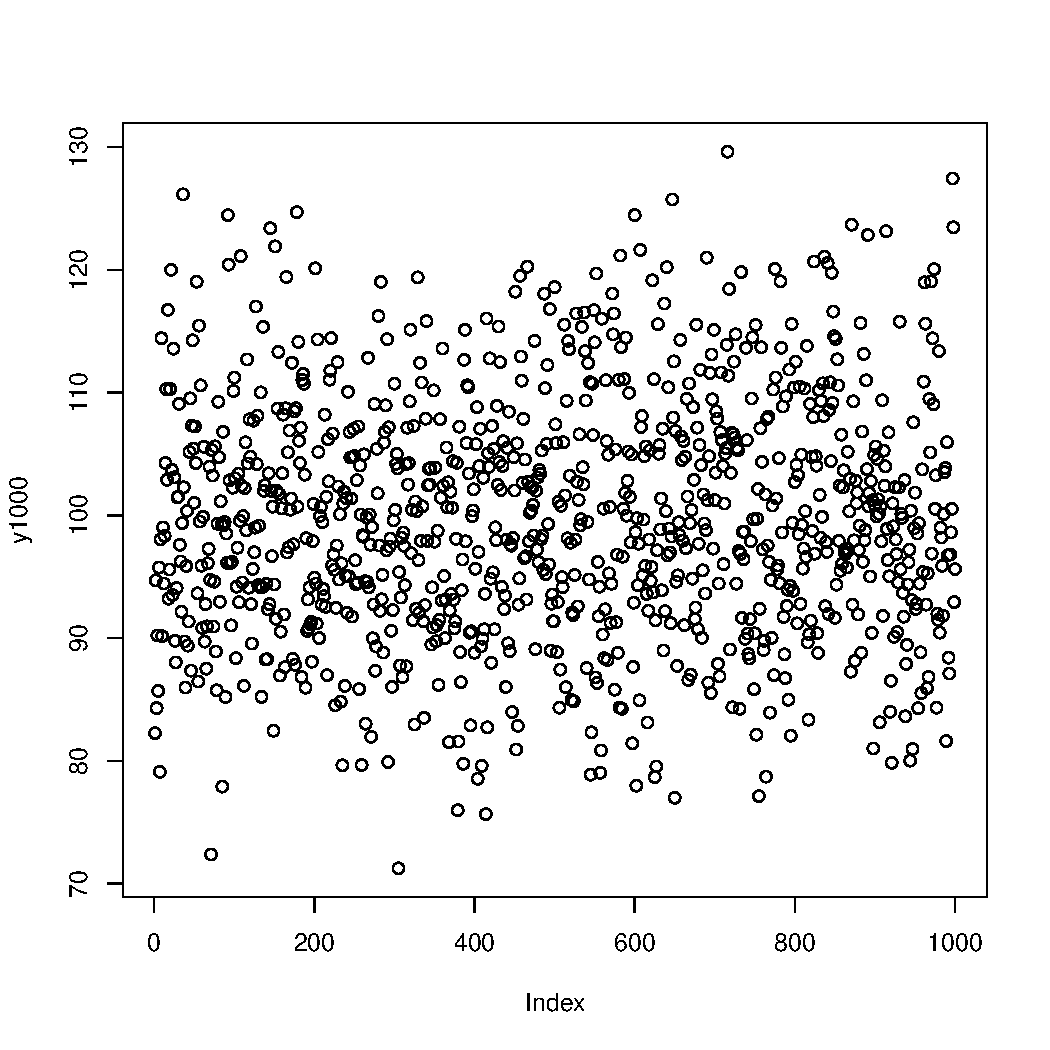
\includegraphics[width=\maxwidth]{figure/unnamed-chunk-11} 
\begin{kframe}\begin{alltt}
\hlkwd{hist}\hlstd{(y1000)}
\end{alltt}
\end{kframe}
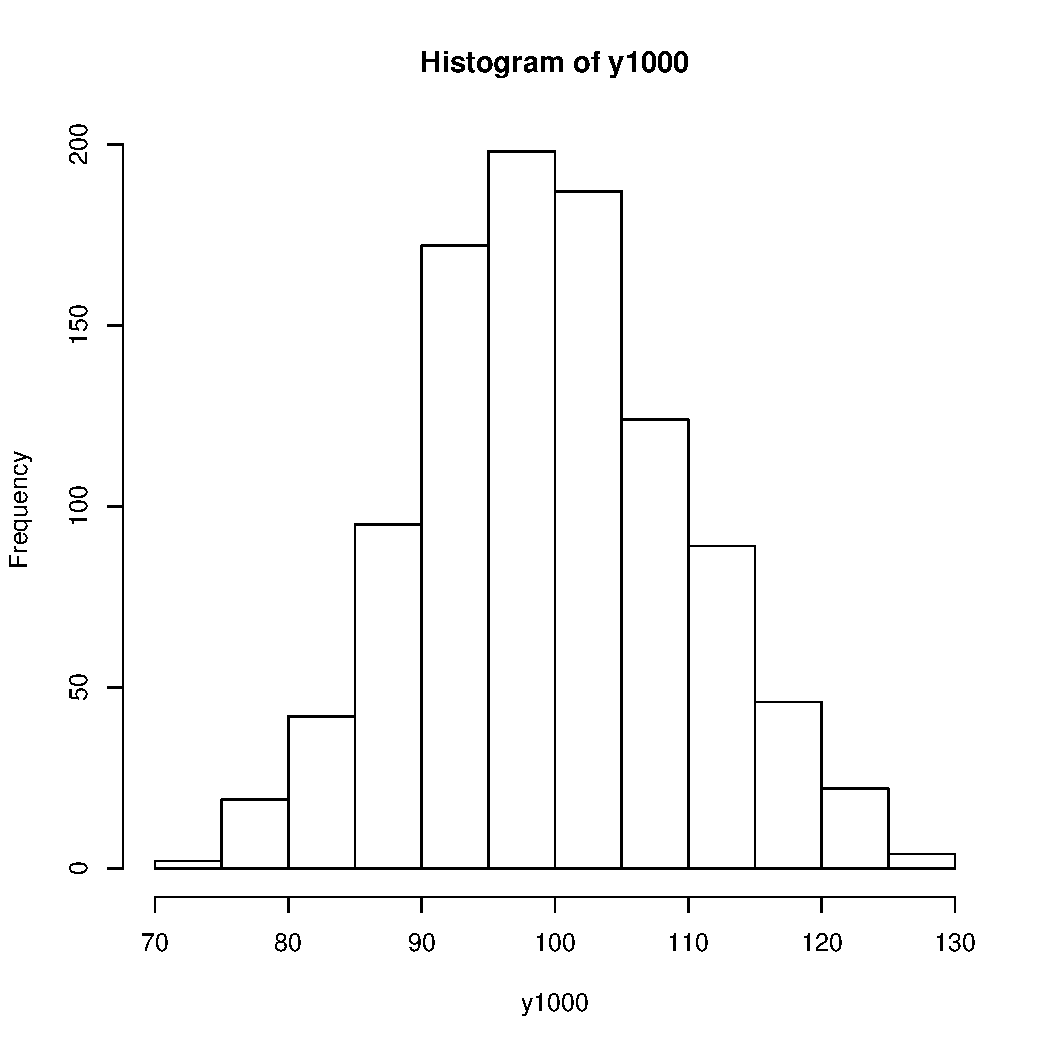
\includegraphics[width=\maxwidth]{figure/unnamed-chunk-12} 
\begin{kframe}\begin{alltt}
\hlcom{## }
\hlkwd{mean}\hlstd{(y1000)}
\end{alltt}
\begin{verbatim}
## [1] 99.73
\end{verbatim}
\begin{alltt}
\hlkwd{sd}\hlstd{(y1000)}
\end{alltt}
\begin{verbatim}
## [1] 9.842
\end{verbatim}
\begin{alltt}
\hlcom{## }
\hlstd{lm0} \hlkwb{<-} \hlkwd{lm}\hlstd{(y1000} \hlopt{~} \hlnum{1}\hlstd{)}
\hlkwd{summary}\hlstd{(lm0)}
\end{alltt}
\begin{verbatim}
## 
## Call:
## lm(formula = y1000 ~ 1)
## 
## Residuals:
##     Min      1Q  Median      3Q     Max 
## -28.477  -6.959  -0.464   6.205  29.901 
## 
## Coefficients:
##             Estimate Std. Error t value Pr(>|t|)    
## (Intercept)   99.728      0.311     320   <2e-16 ***
## ---
## Signif. codes:  0 '***' 0.001 '**' 0.01 '*' 0.05 '.' 0.1 ' ' 1
## 
## Residual standard error: 9.84 on 999 degrees of freedom
\end{verbatim}
\begin{alltt}
## 
\end{alltt}
\end{kframe}
\end{knitrout}


先了解一下密度函数是怎么一回事
\begin{knitrout}
\definecolor{shadecolor}{rgb}{0.969, 0.969, 0.969}\color{fgcolor}\begin{kframe}
\begin{alltt}
\hlkwd{plot}\hlstd{(}\hlkwc{x} \hlstd{=} \hlopt{-}\hlnum{10}\hlopt{:}\hlnum{10}\hlstd{,} \hlkwc{y} \hlstd{=} \hlkwd{dnorm}\hlstd{(}\hlopt{-}\hlnum{10}\hlopt{:}\hlnum{10}\hlstd{,} \hlkwc{mean} \hlstd{=} \hlnum{0}\hlstd{,} \hlkwc{sd} \hlstd{=} \hlnum{1}\hlstd{),} \hlkwc{ylab} \hlstd{=} \hlstr{"Density"}\hlstd{)}
\end{alltt}
\end{kframe}
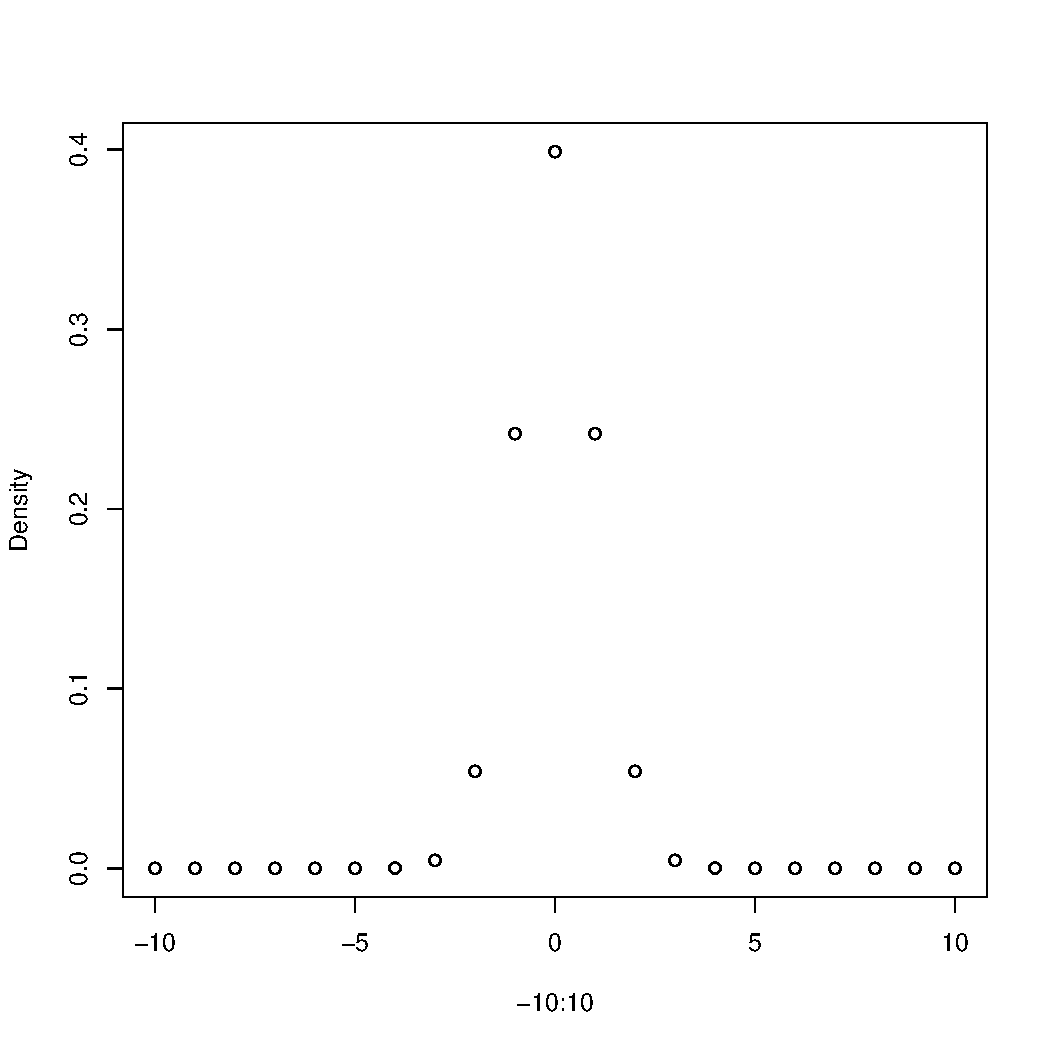
\includegraphics[width=\maxwidth]{figure/unnamed-chunk-21} 
\begin{kframe}\begin{alltt}
\hlkwd{plot}\hlstd{(}\hlkwc{x} \hlstd{=} \hlopt{-}\hlnum{10}\hlopt{:}\hlnum{10}\hlstd{,} \hlkwc{y} \hlstd{=} \hlkwd{dnorm}\hlstd{(}\hlopt{-}\hlnum{10}\hlopt{:}\hlnum{10}\hlstd{,} \hlkwc{mean} \hlstd{=} \hlnum{8}\hlstd{,} \hlkwc{sd} \hlstd{=} \hlnum{1}\hlstd{),} \hlkwc{ylab} \hlstd{=} \hlstr{"Density"}\hlstd{)}
\end{alltt}
\end{kframe}
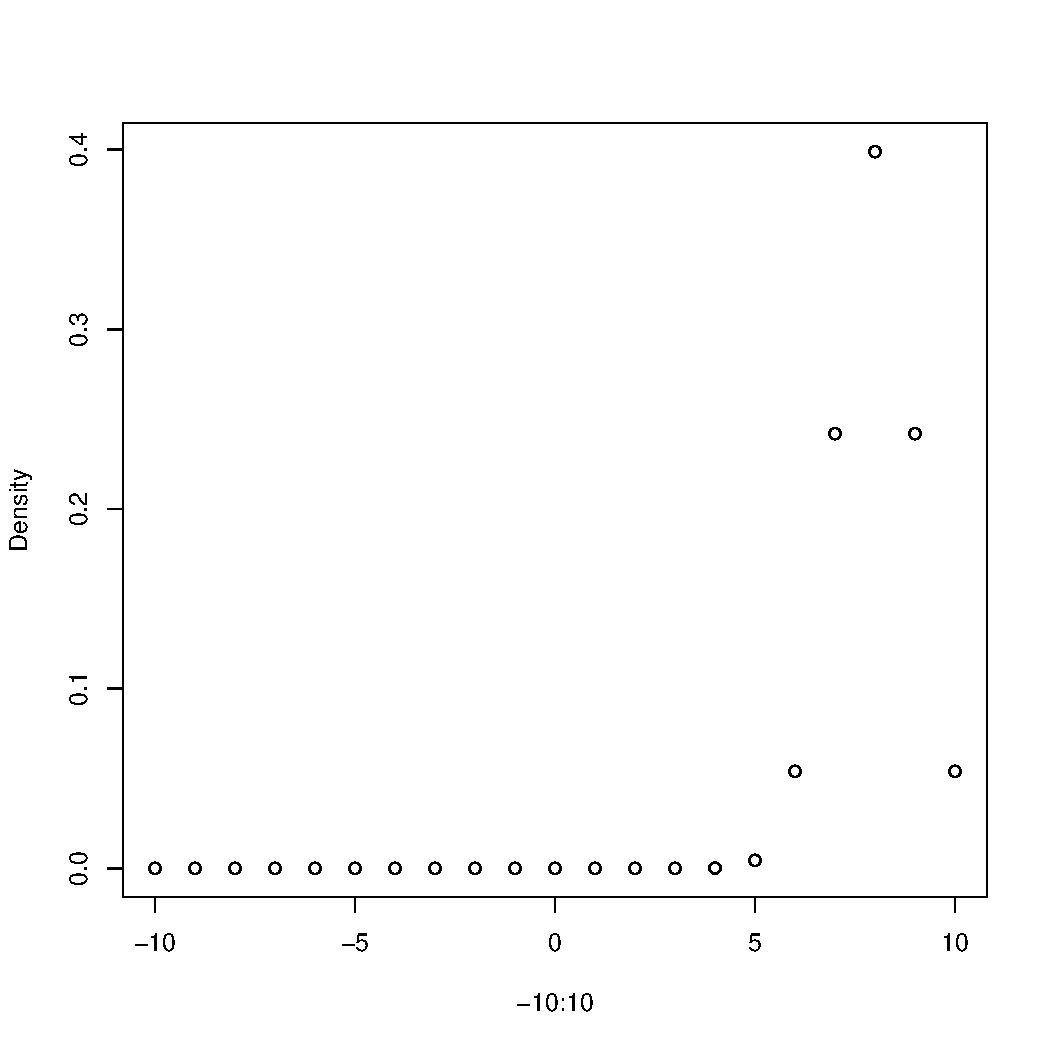
\includegraphics[width=\maxwidth]{figure/unnamed-chunk-22} 
\begin{kframe}\begin{alltt}
\hlkwd{sum}\hlstd{(}\hlkwd{dnorm}\hlstd{(}\hlopt{-}\hlnum{10}\hlopt{:}\hlnum{10}\hlstd{,} \hlkwc{mean} \hlstd{=} \hlnum{0}\hlstd{,} \hlkwc{sd} \hlstd{=} \hlnum{1}\hlstd{))}
\end{alltt}
\begin{verbatim}
## [1] 1
\end{verbatim}
\begin{alltt}
\hlkwd{sum}\hlstd{(}\hlkwd{dnorm}\hlstd{(}\hlopt{-}\hlnum{10}\hlopt{:}\hlnum{10}\hlstd{,} \hlkwc{mean} \hlstd{=} \hlnum{8}\hlstd{,} \hlkwc{sd} \hlstd{=} \hlnum{1}\hlstd{))}
\end{alltt}
\begin{verbatim}
## [1] 0.9954
\end{verbatim}
\begin{alltt}
\hlcom{# }
\hlkwd{plot}\hlstd{(}\hlkwd{dnorm}\hlstd{(}\hlkwd{sample}\hlstd{(}\hlopt{-}\hlnum{10}\hlopt{:}\hlnum{10}\hlstd{)))}
\end{alltt}
\end{kframe}
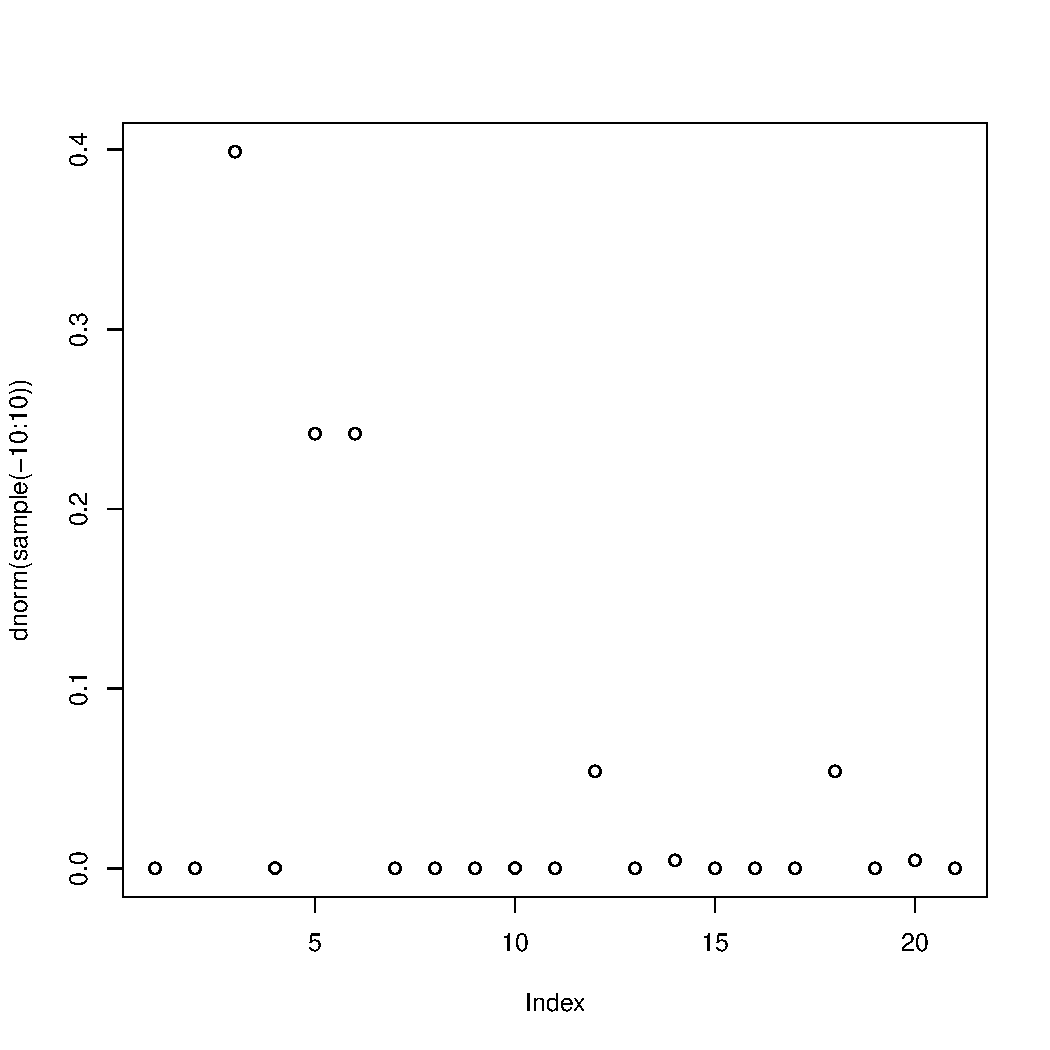
\includegraphics[width=\maxwidth]{figure/unnamed-chunk-23} 

\end{knitrout}


如果假设的正态分布组的方差是1,平均数是1:3000,哪个平均数最有可能,使实际数据的密度函数之和最大呢?
如果假设的正态分布组的平均数是100,方差是1:100,哪个方差最有可能,使实际数据的密度函数之和最大呢?
重复50次之后的结果是不是可靠呢?
\begin{knitrout}
\definecolor{shadecolor}{rgb}{0.969, 0.969, 0.969}\color{fgcolor}\begin{kframe}
\begin{alltt}
\hlstd{population.sd} \hlkwb{<-} \hlnum{1}
\hlkwa{for} \hlstd{(i} \hlkwa{in} \hlnum{1}\hlopt{:}\hlnum{50}\hlstd{) \{}
    \hlstd{mu} \hlkwb{<-} \hlnum{1}\hlopt{:}\hlnum{3000}
    \hlstd{la00} \hlkwb{<-} \hlkwd{sapply}\hlstd{(mu,} \hlkwa{function}\hlstd{(}\hlkwc{xx}\hlstd{)} \hlkwd{sum}\hlstd{(}\hlkwd{dnorm}\hlstd{(y1000, xx, population.sd,} \hlkwc{log} \hlstd{=} \hlnum{TRUE}\hlstd{)))}
    \hlstd{mu} \hlkwb{<-} \hlstd{mu[}\hlkwd{which.max}\hlstd{(la00)]}
    \hlstd{population.sd} \hlkwb{<-} \hlnum{1}\hlopt{:}\hlnum{100}
    \hlstd{d01} \hlkwb{<-} \hlkwd{sapply}\hlstd{(population.sd,} \hlkwa{function}\hlstd{(}\hlkwc{xx}\hlstd{)} \hlkwd{sum}\hlstd{(}\hlkwd{dnorm}\hlstd{(y1000, mu, xx,} \hlkwc{log} \hlstd{=} \hlnum{TRUE}\hlstd{)))}
    \hlstd{population.sd} \hlkwb{<-} \hlstd{population.sd[}\hlkwd{which.max}\hlstd{(d01)]}
\hlstd{\}}
\hlkwd{c}\hlstd{(}\hlkwc{mean} \hlstd{= mu,} \hlkwc{sd} \hlstd{= population.sd)}
\end{alltt}
\begin{verbatim}
## mean   sd 
##  100   10
\end{verbatim}
\begin{alltt}
\hlcom{# }
\hlkwd{plot}\hlstd{(la00)}
\end{alltt}
\end{kframe}
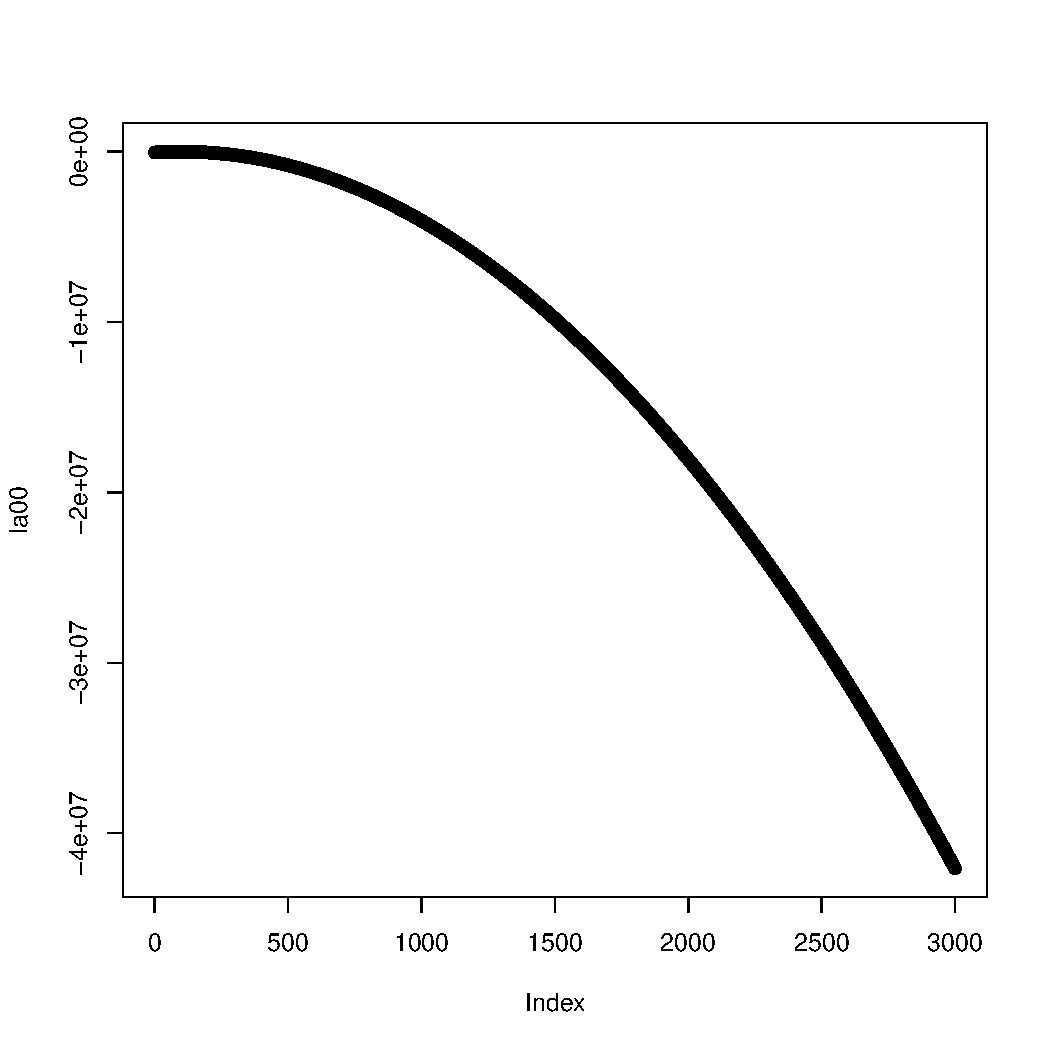
\includegraphics[width=\maxwidth]{figure/unnamed-chunk-31} 
\begin{kframe}\begin{alltt}
\hlkwd{plot}\hlstd{(d01)}
\end{alltt}
\end{kframe}
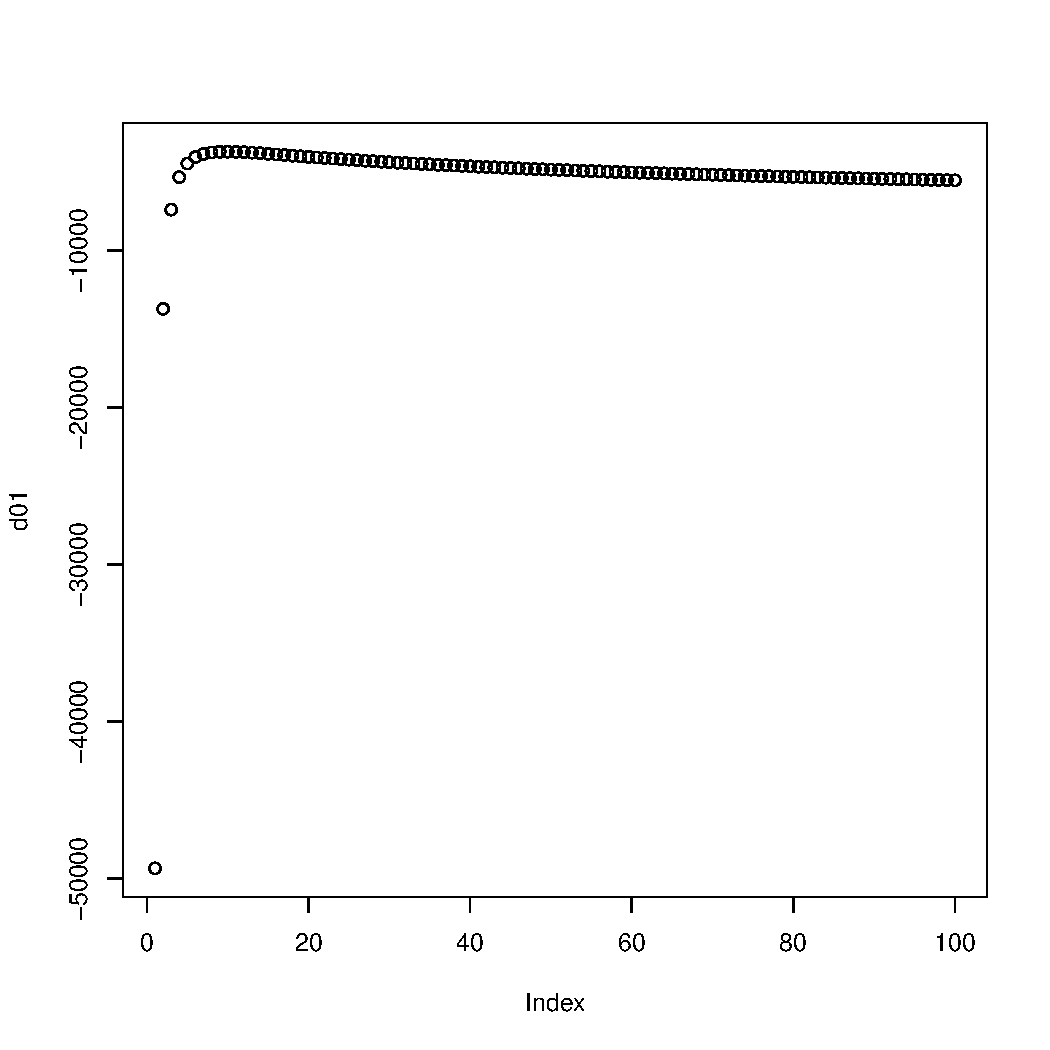
\includegraphics[width=\maxwidth]{figure/unnamed-chunk-32} 

\end{knitrout}


来看看R语言的LaplacesDemon包是怎么将暴力进行到底的呢?
Model function 就相当于一个for循环。那么就让Model循环10000次吧。

\begin{knitrout}
\definecolor{shadecolor}{rgb}{0.969, 0.969, 0.969}\color{fgcolor}\begin{kframe}
\begin{alltt}
\hlcom{# Load library}
\hlkwd{library}\hlstd{(LaplacesDemon)}
\end{alltt}


{\ttfamily\noindent\itshape\color{messagecolor}{\#\# Loading required package: parallel}}\begin{alltt}
\hlstd{y1000} \hlkwb{<-} \hlkwd{rnorm}\hlstd{(}\hlkwc{n} \hlstd{=} \hlnum{1000}\hlstd{,} \hlkwc{mean} \hlstd{=} \hlnum{250}\hlstd{,} \hlkwc{sd} \hlstd{=} \hlnum{10}\hlstd{)}  \hlcom{# Sample of 1000 birds}
\hlcom{## Model specification}
\hlstd{Model} \hlkwb{<-} \hlkwa{function}\hlstd{(}\hlkwc{parm}\hlstd{,} \hlkwc{Data}\hlstd{) \{}
    \hlcom{# Parameters}
    \hlstd{population.mean} \hlkwb{<-} \hlstd{parm[}\hlnum{1}\hlstd{]}
    \hlstd{population.sd} \hlkwb{<-} \hlstd{parm[}\hlnum{2}\hlstd{]}
    \hlcom{# Prior density}
    \hlstd{population.mean.prior} \hlkwb{<-} \hlkwd{dunif}\hlstd{(population.mean,} \hlnum{0}\hlstd{,} \hlnum{5000}\hlstd{)}
    \hlstd{population.sd.prior} \hlkwb{<-} \hlkwd{dunif}\hlstd{(population.sd,} \hlnum{0}\hlstd{,} \hlnum{100}\hlstd{)}
    \hlcom{# Log-Likelihood}
    \hlstd{mu} \hlkwb{<-} \hlstd{population.mean}
    \hlstd{LL} \hlkwb{<-} \hlkwd{sum}\hlstd{(}\hlkwd{dnorm}\hlstd{(Data}\hlopt{$}\hlstd{mass, mu, population.sd,} \hlkwc{log} \hlstd{=} \hlnum{TRUE}\hlstd{))}
    \hlcom{# Log-Posterior}
    \hlstd{LP} \hlkwb{<-} \hlstd{LL} \hlopt{+} \hlstd{population.mean.prior} \hlopt{+} \hlstd{population.sd.prior}
    \hlstd{Modelout} \hlkwb{<-} \hlkwd{list}\hlstd{(}\hlkwc{LP} \hlstd{= LP,} \hlkwc{Dev} \hlstd{=} \hlopt{-}\hlnum{2} \hlopt{*} \hlstd{LL,} \hlkwc{Monitor} \hlstd{=} \hlkwd{c}\hlstd{(LP),} \hlkwc{yhat} \hlstd{=} \hlkwd{rnorm}\hlstd{(Data}\hlopt{$}\hlstd{N,}
        \hlstd{mu, population.sd),} \hlkwc{parm} \hlstd{= parm)}
    \hlkwd{return}\hlstd{(Modelout)}
\hlstd{\}}
\hlcom{# Prepare the data}
\hlstd{parm.names} \hlkwb{<-} \hlkwd{c}\hlstd{(}\hlstr{"population.mean0"}\hlstd{,} \hlstr{"population.sd0"}\hlstd{)}
\hlstd{Data} \hlkwb{<-} \hlkwd{list}\hlstd{(}\hlkwc{mass} \hlstd{= y1000,} \hlkwc{N} \hlstd{=} \hlkwd{length}\hlstd{(y1000),} \hlkwc{mon.names} \hlstd{=} \hlkwd{c}\hlstd{(}\hlstr{"LP"}\hlstd{),} \hlkwc{parm.names} \hlstd{= parm.names)}
\hlcom{# Initial values}
\hlstd{Initial.Values} \hlkwb{<-} \hlkwd{c}\hlstd{(}\hlnum{1000}\hlstd{,} \hlopt{-}\hlnum{250}\hlstd{)}
\hlcom{# MCMC settings}
\hlstd{ni} \hlkwb{<-} \hlnum{5000}  \hlcom{# Number of draws from posterior (for each chain)}
\hlstd{st} \hlkwb{<-} \hlnum{1000}  \hlcom{# Steps when status message should be given}
\hlstd{nt} \hlkwb{<-} \hlnum{50}  \hlcom{# Thinning rate #  Abate autocorrelation}
\hlcom{# Run LaplacesDemon}
\hlstd{out} \hlkwb{<-} \hlkwd{LaplacesDemon}\hlstd{(Model,} \hlkwc{Data} \hlstd{= Data, Initial.Values,} \hlkwc{Iterations} \hlstd{= ni,} \hlkwc{Status} \hlstd{= st,}
    \hlkwc{Thinning} \hlstd{= nt)}
\end{alltt}
\begin{verbatim}
## 
## Laplace's Demon was called on Wed Oct 30 18:04:56 2013
## 
## Performing initial checks...
\end{verbatim}


{\ttfamily\noindent\color{warningcolor}{\#\# Warning: NaNs produced\\\#\# Warning: NAs produced}}\begin{verbatim}
## Generating initial values due to a non-finite posterior.
\end{verbatim}


{\ttfamily\noindent\color{warningcolor}{\#\# Warning: NaNs produced\\\#\# Warning: NAs produced\\\#\# Warning: NaNs produced\\\#\# Warning: NAs produced\\\#\# Warning: NaNs produced\\\#\# Warning: NAs produced\\\#\# Warning: NaNs produced\\\#\# Warning: NAs produced}}\begin{verbatim}
## Algorithm: Random-Walk Metropolis 
## 
## Laplace's Demon is beginning to update...
## Iteration: 1000,   Proposal: Multivariate
## Iteration: 2000,   Proposal: Multivariate
## Iteration: 3000,   Proposal: Multivariate
## Iteration: 4000,   Proposal: Multivariate
## Iteration: 5000,   Proposal: Multivariate
## 
## Assessing Stationarity
## Assessing Thinning and ESS
## Creating Summaries
## Estimating Log of the Marginal Likelihood
## 
## WARNING: At least 301 samples are required for NSIS.
## Creating Output
## 
## Laplace's Demon has finished.
\end{verbatim}
\begin{alltt}
\hlcom{# Have a look at some summary statistics}
\hlstd{out}
\end{alltt}
\begin{verbatim}
## Call:
## LaplacesDemon(Model = Model, Data = Data, Initial.Values = Initial.Values, 
##     Iterations = ni, Status = st, Thinning = nt)
## 
## Acceptance Rate: 0.094
## Adaptive: 5001
## Algorithm: Random-Walk Metropolis
## Covariance Matrix: (NOT SHOWN HERE; diagonal shown instead)
## population.mean0   population.sd0 
##            2.835            2.835 
## 
## Covariance (Diagonal) History: (NOT SHOWN HERE)
## Deviance Information Criterion (DIC):
##          All Stationary
## Dbar    7956     7449.2
## pD   1433069      278.3
## DIC  1441024     7727.5
## 
## Delayed Rejection (DR): 0
## Initial Values:
## [1] 42.79 51.29
## 
## Iterations: 5000
## Log(Marginal Likelihood): NA
## Minutes of run-time: 0.02
## Model: (NOT SHOWN HERE)
## Monitor: (NOT SHOWN HERE)
## Parameters (Number of): 2
## Periodicity: 5001
## Posterior1: (NOT SHOWN HERE)
## Posterior2: (NOT SHOWN HERE)
## Recommended Burn-In of Thinned Samples: 10
## Recommended Burn-In of Un-thinned Samples: 500
## Recommended Thinning: 400
## Status is displayed every 1000 iterations
## Summary1: (SHOWN BELOW)
## Summary2: (SHOWN BELOW)
## Thinned Samples: 100
## Thinning: 50
## 
## 
## Summary of All Samples
##                      Mean      SD   MCSE    ESS        LB  Median      UB
## population.mean0   239.16   39.27  14.56  7.461    86.407   250.2   250.8
## population.sd0      18.86   28.52  11.47 12.477     9.633    10.1   118.7
## Deviance          7955.58 1692.97 666.52 11.773  7444.874  7446.4 13105.7
## LP               -3977.78  846.49 333.26 11.773 -6552.836 -3723.2 -3722.4
## 
## 
## Summary of Stationary Samples
##                      Mean      SD      MCSE ESS        LB   Median
## population.mean0   250.23  0.4124   0.04023  90   249.668   250.22
## population.sd0      10.11  0.4844   0.05074  90     9.624    10.06
## Deviance          7449.19 23.5941   2.45715  90  7444.873  7446.20
## LP               -3724.59 11.7971 333.26228  90 -3726.344 -3723.09
##                        UB
## population.mean0   250.78
## population.sd0      10.58
## Deviance          7452.71
## LP               -3722.43
\end{verbatim}
\begin{alltt}
\hlcom{# Plotting output}
\hlkwd{plot}\hlstd{(out,} \hlkwc{BurnIn} \hlstd{=} \hlnum{50}\hlstd{, Data,} \hlkwc{Parms} \hlstd{= (}\hlstr{".mean0"}\hlstd{))}
\end{alltt}
\end{kframe}
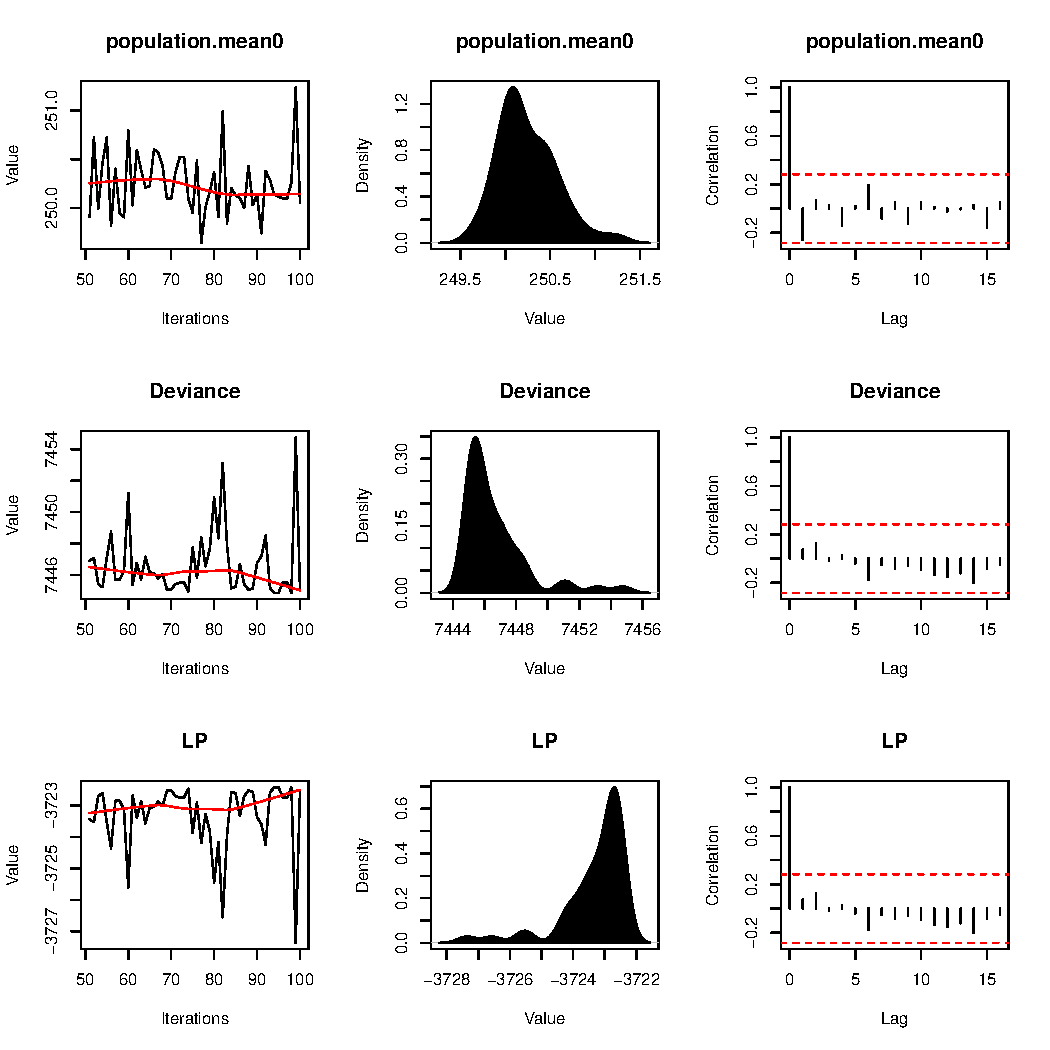
\includegraphics[width=\maxwidth]{figure/unnamed-chunk-4} 
\begin{kframe}\begin{alltt}

\end{alltt}
\end{kframe}
\end{knitrout}


第二章: 关于平均值、T检验、线性回归、单变量方差分析、双变量方差分析、协方差分析
  
数据:
mass生物量, pop种群, region范围, hab栖息地, svl体长
\begin{knitrout}
\definecolor{shadecolor}{rgb}{0.969, 0.969, 0.969}\color{fgcolor}\begin{kframe}
\begin{alltt}
\hlstd{mass} \hlkwb{<-} \hlkwd{c}\hlstd{(}\hlnum{6}\hlstd{,} \hlnum{8}\hlstd{,} \hlnum{5}\hlstd{,} \hlnum{7}\hlstd{,} \hlnum{9}\hlstd{,} \hlnum{11}\hlstd{)}
\hlstd{pop} \hlkwb{<-} \hlkwd{factor}\hlstd{(}\hlkwd{c}\hlstd{(}\hlnum{1}\hlstd{,} \hlnum{1}\hlstd{,} \hlnum{2}\hlstd{,} \hlnum{2}\hlstd{,} \hlnum{3}\hlstd{,} \hlnum{3}\hlstd{))}
\hlstd{region} \hlkwb{<-} \hlkwd{factor}\hlstd{(}\hlkwd{c}\hlstd{(}\hlnum{1}\hlstd{,} \hlnum{1}\hlstd{,} \hlnum{1}\hlstd{,} \hlnum{1}\hlstd{,} \hlnum{2}\hlstd{,} \hlnum{2}\hlstd{))}
\hlstd{hab} \hlkwb{<-} \hlkwd{factor}\hlstd{(}\hlkwd{c}\hlstd{(}\hlnum{1}\hlstd{,} \hlnum{2}\hlstd{,} \hlnum{3}\hlstd{,} \hlnum{1}\hlstd{,} \hlnum{2}\hlstd{,} \hlnum{3}\hlstd{))}
\hlstd{svl} \hlkwb{<-} \hlkwd{c}\hlstd{(}\hlnum{40}\hlstd{,} \hlnum{45}\hlstd{,} \hlnum{39}\hlstd{,} \hlnum{50}\hlstd{,} \hlnum{52}\hlstd{,} \hlnum{57}\hlstd{)}
\end{alltt}
\end{kframe}
\end{knitrout}

平均值:
 mass_i =μ+ε_i ,    εi~Normal(0,σ^2)
\begin{knitrout}
\definecolor{shadecolor}{rgb}{0.969, 0.969, 0.969}\color{fgcolor}\begin{kframe}
\begin{alltt}
\hlcom{# mean}
\hlkwd{lm}\hlstd{(mass} \hlopt{~} \hlnum{1}\hlstd{)}  \hlcom{#  massi =μ+εi ,    εi~Normal(0,σ^2)}
\end{alltt}
\begin{verbatim}
## 
## Call:
## lm(formula = mass ~ 1)
## 
## Coefficients:
## (Intercept)  
##        7.67
\end{verbatim}
\begin{alltt}
\hlkwd{model.matrix}\hlstd{(mass} \hlopt{~} \hlnum{1}\hlstd{)}
\end{alltt}
\begin{verbatim}
##   (Intercept)
## 1           1
## 2           1
## 3           1
## 4           1
## 5           1
## 6           1
## attr(,"assign")
## [1] 0
\end{verbatim}
\end{kframe}
\end{knitrout}


t检验:
 mass_i = α + β * region_i + ε_i; ε_i ~ Normal(0, σ^2)
 mass_i ~ Normal(α + β * region, σ^2)
 
c(6, 8, 5, 7, 9, 11) = α * (1, 1, 1, 1, 1, 1) + β * factor(c(1,1,1,1,2,2)) + c(ε1,ε2,ε3,ε4,ε5,ε6)

\begin{knitrout}
\definecolor{shadecolor}{rgb}{0.969, 0.969, 0.969}\color{fgcolor}\begin{kframe}
\begin{alltt}
\hlcom{# t-test}
\hlkwd{lm}\hlstd{(mass} \hlopt{~} \hlstd{region)}  \hlcom{# }
\end{alltt}
\begin{verbatim}
## 
## Call:
## lm(formula = mass ~ region)
## 
## Coefficients:
## (Intercept)      region2  
##         6.5          3.5
\end{verbatim}
\begin{alltt}
\hlkwd{model.matrix}\hlstd{(}\hlopt{~}\hlstd{region)}
\end{alltt}
\begin{verbatim}
##   (Intercept) region2
## 1           1       0
## 2           1       0
## 3           1       0
## 4           1       0
## 5           1       1
## 6           1       1
## attr(,"assign")
## [1] 0 1
## attr(,"contrasts")
## attr(,"contrasts")$region
## [1] "contr.treatment"
\end{verbatim}
\begin{alltt}
\hlkwd{summary}\hlstd{(}\hlkwd{lm}\hlstd{(mass} \hlopt{~} \hlstd{region))}
\end{alltt}
\begin{verbatim}
## 
## Call:
## lm(formula = mass ~ region)
## 
## Residuals:
##    1    2    3    4    5    6 
## -0.5  1.5 -1.5  0.5 -1.0  1.0 
## 
## Coefficients:
##             Estimate Std. Error t value Pr(>|t|)    
## (Intercept)    6.500      0.661    9.83   0.0006 ***
## region2        3.500      1.146    3.06   0.0378 *  
## ---
## Signif. codes:  0 '***' 0.001 '**' 0.01 '*' 0.05 '.' 0.1 ' ' 1
## 
## Residual standard error: 1.32 on 4 degrees of freedom
## Multiple R-squared:   0.7,	Adjusted R-squared:  0.625 
## F-statistic: 9.33 on 1 and 4 DF,  p-value: 0.0378
\end{verbatim}
\begin{alltt}
\hlcom{# mass_i =α+β*region_i+ε_i ε_i~Normal(0,σ^2) mass_i~Normal(α+β*region,σ^2)}
\hlcom{# c(6, 8, 5, 7, 9, 11) = α * (1, 1, 1, 1, 1, 1) + β * factor(c(1,1,1,1,2,2))}
\hlcom{# + c(ε1,ε2,ε3,ε4,ε5,ε6)}
\hlkwd{lm}\hlstd{(mass} \hlopt{~} \hlstd{region} \hlopt{-} \hlnum{1}\hlstd{)}
\end{alltt}
\begin{verbatim}
## 
## Call:
## lm(formula = mass ~ region - 1)
## 
## Coefficients:
## region1  region2  
##     6.5     10.0
\end{verbatim}
\begin{alltt}
\hlkwd{model.matrix}\hlstd{(}\hlopt{~}\hlstd{region} \hlopt{-} \hlnum{1}\hlstd{)}
\end{alltt}
\begin{verbatim}
##   region1 region2
## 1       1       0
## 2       1       0
## 3       1       0
## 4       1       0
## 5       0       1
## 6       0       1
## attr(,"assign")
## [1] 1 1
## attr(,"contrasts")
## attr(,"contrasts")$region
## [1] "contr.treatment"
\end{verbatim}
\begin{alltt}
\hlkwd{summary}\hlstd{(}\hlkwd{lm}\hlstd{(mass} \hlopt{~} \hlstd{region} \hlopt{-} \hlnum{1}\hlstd{))}
\end{alltt}
\begin{verbatim}
## 
## Call:
## lm(formula = mass ~ region - 1)
## 
## Residuals:
##    1    2    3    4    5    6 
## -0.5  1.5 -1.5  0.5 -1.0  1.0 
## 
## Coefficients:
##         Estimate Std. Error t value Pr(>|t|)    
## region1    6.500      0.661    9.83  0.00060 ***
## region2   10.000      0.935   10.69  0.00043 ***
## ---
## Signif. codes:  0 '***' 0.001 '**' 0.01 '*' 0.05 '.' 0.1 ' ' 1
## 
## Residual standard error: 1.32 on 4 degrees of freedom
## Multiple R-squared:  0.981,	Adjusted R-squared:  0.972 
## F-statistic:  105 on 2 and 4 DF,  p-value: 0.000347
\end{verbatim}
\begin{alltt}
# 6.5 + 3.5 = 10.0
\end{alltt}
\end{kframe}
\end{knitrout}


简单线性回归:
 mass_i = α + β * svl_i + ε_i; ε_i ~ Normal(0, σ^2)
 mass_i ~ Normal(α + β * svl_i, σ^2)
\begin{knitrout}
\definecolor{shadecolor}{rgb}{0.969, 0.969, 0.969}\color{fgcolor}\begin{kframe}
\begin{alltt}
\hlkwd{lm}\hlstd{(mass} \hlopt{~} \hlstd{svl)}
\end{alltt}
\begin{verbatim}
## 
## Call:
## lm(formula = mass ~ svl)
## 
## Coefficients:
## (Intercept)          svl  
##       -5.56         0.28
\end{verbatim}
\begin{alltt}
\hlkwd{model.matrix}\hlstd{(}\hlopt{~}\hlstd{svl)}
\end{alltt}
\begin{verbatim}
##   (Intercept) svl
## 1           1  40
## 2           1  45
## 3           1  39
## 4           1  50
## 5           1  52
## 6           1  57
## attr(,"assign")
## [1] 0 1
\end{verbatim}
\begin{alltt}
\hlcom{# }
\hlkwd{lm}\hlstd{(mass} \hlopt{~} \hlstd{svl} \hlopt{-} \hlnum{1}\hlstd{)}
\end{alltt}
\begin{verbatim}
## 
## Call:
## lm(formula = mass ~ svl - 1)
## 
## Coefficients:
##   svl  
## 0.165
\end{verbatim}
\begin{alltt}
\hlkwd{model.matrix}\hlstd{(}\hlopt{~}\hlstd{svl} \hlopt{-} \hlnum{1}\hlstd{)}
\end{alltt}
\begin{verbatim}
##   svl
## 1  40
## 2  45
## 3  39
## 4  50
## 5  52
## 6  57
## attr(,"assign")
## [1] 1
\end{verbatim}
\end{kframe}
\end{knitrout}


单变量方差分解:

 β.j_i是第j组pop以及第i个个体的参数。
 mass_i = α + β.j_i * pop_i + ε_i; ε_i ~ Normal(0, σ^2)
 mass_i ~ Normal(α + β.j_i * pop_i, σ^2)
 
 Each parameterization is better suited to a different aim: the effects
model is better for testing for differences and the means model is better
for presentation.

\begin{knitrout}
\definecolor{shadecolor}{rgb}{0.969, 0.969, 0.969}\color{fgcolor}\begin{kframe}
\begin{alltt}
\hlcom{# effects model}
\hlkwd{lm}\hlstd{(mass} \hlopt{~} \hlstd{pop)}
\end{alltt}
\begin{verbatim}
## 
## Call:
## lm(formula = mass ~ pop)
## 
## Coefficients:
## (Intercept)         pop2         pop3  
##           7           -1            3
\end{verbatim}
\begin{alltt}
\hlkwd{model.matrix}\hlstd{(}\hlopt{~}\hlstd{pop)}
\end{alltt}
\begin{verbatim}
##   (Intercept) pop2 pop3
## 1           1    0    0
## 2           1    0    0
## 3           1    1    0
## 4           1    1    0
## 5           1    0    1
## 6           1    0    1
## attr(,"assign")
## [1] 0 1 1
## attr(,"contrasts")
## attr(,"contrasts")$pop
## [1] "contr.treatment"
\end{verbatim}
\begin{alltt}
\hlcom{# means model}
\hlkwd{lm}\hlstd{(mass} \hlopt{~} \hlstd{pop} \hlopt{-} \hlnum{1}\hlstd{)}
\end{alltt}
\begin{verbatim}
## 
## Call:
## lm(formula = mass ~ pop - 1)
## 
## Coefficients:
## pop1  pop2  pop3  
##    7     6    10
\end{verbatim}
\begin{alltt}
\hlkwd{model.matrix}\hlstd{(}\hlopt{~}\hlstd{pop} \hlopt{-} \hlnum{1}\hlstd{)}
\end{alltt}
\begin{verbatim}
##   pop1 pop2 pop3
## 1    1    0    0
## 2    1    0    0
## 3    0    1    0
## 4    0    1    0
## 5    0    0    1
## 6    0    0    1
## attr(,"assign")
## [1] 1 1 1
## attr(,"contrasts")
## attr(,"contrasts")$pop
## [1] "contr.treatment"
\end{verbatim}
\end{kframe}
\end{knitrout}



双变量方差分解:two-way analysis of variance

model 1:
mass_i = α + β_j.i * region_i + δ_k.i * hab_i + ε_i;
      ε_i ~ Normal(0, σ^2)

model 2:
mass_i = α + β_j.i * region_i + δ_k.i * hab_i 
         + γ_j.k.i * region_i * hab_i + ε_i;
      ε_i ~ Normal(0, σ^2)

model 3:
mass_i = α_j.k.i * region_i * hab_i + ε_i;
      ε_i ~ Normal(0, σ^2)
      
\begin{knitrout}
\definecolor{shadecolor}{rgb}{0.969, 0.969, 0.969}\color{fgcolor}\begin{kframe}
\begin{alltt}
\hlkwd{lm}\hlstd{(mass} \hlopt{~} \hlstd{region} \hlopt{+} \hlstd{hab)}
\end{alltt}
\begin{verbatim}
## 
## Call:
## lm(formula = mass ~ region + hab)
## 
## Coefficients:
## (Intercept)      region2         hab2         hab3  
##        6.50         3.50         0.25        -0.25
\end{verbatim}
\begin{alltt}
\hlkwd{model.matrix}\hlstd{(}\hlopt{~}\hlstd{region} \hlopt{+} \hlstd{hab)}  \hlcom{# model 1}
\end{alltt}
\begin{verbatim}
##   (Intercept) region2 hab2 hab3
## 1           1       0    0    0
## 2           1       0    1    0
## 3           1       0    0    1
## 4           1       0    0    0
## 5           1       1    1    0
## 6           1       1    0    1
## attr(,"assign")
## [1] 0 1 2 2
## attr(,"contrasts")
## attr(,"contrasts")$region
## [1] "contr.treatment"
## 
## attr(,"contrasts")$hab
## [1] "contr.treatment"
\end{verbatim}
\begin{alltt}
\hlcom{# }
\hlkwd{lm}\hlstd{(mass} \hlopt{~} \hlstd{region} \hlopt{*} \hlstd{hab)}
\end{alltt}
\begin{verbatim}
## 
## Call:
## lm(formula = mass ~ region * hab)
## 
## Coefficients:
##  (Intercept)       region2          hab2          hab3  region2:hab2  
##          6.5           6.0           1.5          -1.5          -5.0  
## region2:hab3  
##           NA
\end{verbatim}
\begin{alltt}
\hlkwd{model.matrix}\hlstd{(}\hlopt{~}\hlstd{region} \hlopt{*} \hlstd{hab)}  \hlcom{# model 2}
\end{alltt}
\begin{verbatim}
##   (Intercept) region2 hab2 hab3 region2:hab2 region2:hab3
## 1           1       0    0    0            0            0
## 2           1       0    1    0            0            0
## 3           1       0    0    1            0            0
## 4           1       0    0    0            0            0
## 5           1       1    1    0            1            0
## 6           1       1    0    1            0            1
## attr(,"assign")
## [1] 0 1 2 2 3 3
## attr(,"contrasts")
## attr(,"contrasts")$region
## [1] "contr.treatment"
## 
## attr(,"contrasts")$hab
## [1] "contr.treatment"
\end{verbatim}
\begin{alltt}
\hlcom{# }
\hlkwd{lm}\hlstd{(mass} \hlopt{~} \hlstd{region} \hlopt{*} \hlstd{hab} \hlopt{-} \hlnum{1} \hlopt{-} \hlstd{region} \hlopt{-} \hlstd{hab)}
\end{alltt}
\begin{verbatim}
## 
## Call:
## lm(formula = mass ~ region * hab - 1 - region - hab)
## 
## Coefficients:
## region1:hab1  region2:hab1  region1:hab2  region2:hab2  region1:hab3  
##          6.5            NA           8.0           9.0           5.0  
## region2:hab3  
##         11.0
\end{verbatim}
\begin{alltt}
\hlkwd{model.matrix}\hlstd{(}\hlopt{~}\hlstd{region} \hlopt{*} \hlstd{hab} \hlopt{-} \hlnum{1} \hlopt{-} \hlstd{region} \hlopt{-} \hlstd{hab)}  \hlcom{# model 3}
\end{alltt}
\begin{verbatim}
##   region1:hab1 region2:hab1 region1:hab2 region2:hab2 region1:hab3
## 1            1            0            0            0            0
## 2            0            0            1            0            0
## 3            0            0            0            0            1
## 4            1            0            0            0            0
## 5            0            0            0            1            0
## 6            0            0            0            0            0
##   region2:hab3
## 1            0
## 2            0
## 3            0
## 4            0
## 5            0
## 6            1
## attr(,"assign")
## [1] 1 1 1 1 1 1
## attr(,"contrasts")
## attr(,"contrasts")$region
## [1] "contr.treatment"
## 
## attr(,"contrasts")$hab
## [1] "contr.treatment"
\end{verbatim}
\end{kframe}
\end{knitrout}



协方差分析:analysis of covariance
\begin{knitrout}
\definecolor{shadecolor}{rgb}{0.969, 0.969, 0.969}\color{fgcolor}\begin{kframe}
\begin{alltt}
\hlcom{# }
\hlstd{fm} \hlkwb{<-} \hlkwd{lm}\hlstd{(mass} \hlopt{~} \hlstd{pop} \hlopt{+} \hlstd{svl)}  \hlcom{# Refit model}
\hlstd{fm}
\end{alltt}
\begin{verbatim}
## 
## Call:
## lm(formula = mass ~ pop + svl)
## 
## Coefficients:
## (Intercept)         pop2         pop3          svl  
##     -3.4386      -1.4912       0.0526       0.2456
\end{verbatim}
\begin{alltt}
\hlkwd{model.matrix}\hlstd{(}\hlopt{~}\hlstd{pop} \hlopt{+} \hlstd{svl)}
\end{alltt}
\begin{verbatim}
##   (Intercept) pop2 pop3 svl
## 1           1    0    0  40
## 2           1    0    0  45
## 3           1    1    0  39
## 4           1    1    0  50
## 5           1    0    1  52
## 6           1    0    1  57
## attr(,"assign")
## [1] 0 1 1 2
## attr(,"contrasts")
## attr(,"contrasts")$pop
## [1] "contr.treatment"
\end{verbatim}
\begin{alltt}
\hlkwd{plot}\hlstd{(svl, mass,} \hlkwc{col} \hlstd{=} \hlkwd{c}\hlstd{(}\hlkwd{rep}\hlstd{(}\hlstr{"red"}\hlstd{,} \hlnum{2}\hlstd{),} \hlkwd{rep}\hlstd{(}\hlstr{"blue"}\hlstd{,} \hlnum{2}\hlstd{),} \hlkwd{rep}\hlstd{(}\hlstr{"green"}\hlstd{,} \hlnum{2}\hlstd{)))}
\hlkwd{abline}\hlstd{(fm}\hlopt{$}\hlstd{coef[}\hlnum{1}\hlstd{], fm}\hlopt{$}\hlstd{coef[}\hlnum{4}\hlstd{],} \hlkwc{col} \hlstd{=} \hlstr{"red"}\hlstd{)}
\hlkwd{abline}\hlstd{(fm}\hlopt{$}\hlstd{coef[}\hlnum{1}\hlstd{]} \hlopt{+} \hlstd{fm}\hlopt{$}\hlstd{coef[}\hlnum{2}\hlstd{], fm}\hlopt{$}\hlstd{coef[}\hlnum{4}\hlstd{],} \hlkwc{col} \hlstd{=} \hlstr{"blue"}\hlstd{)}
\hlkwd{abline}\hlstd{(fm}\hlopt{$}\hlstd{coef[}\hlnum{1}\hlstd{]} \hlopt{+} \hlstd{fm}\hlopt{$}\hlstd{coef[}\hlnum{3}\hlstd{], fm}\hlopt{$}\hlstd{coef[}\hlnum{4}\hlstd{],} \hlkwc{col} \hlstd{=} \hlstr{"green"}\hlstd{)}
\end{alltt}
\end{kframe}
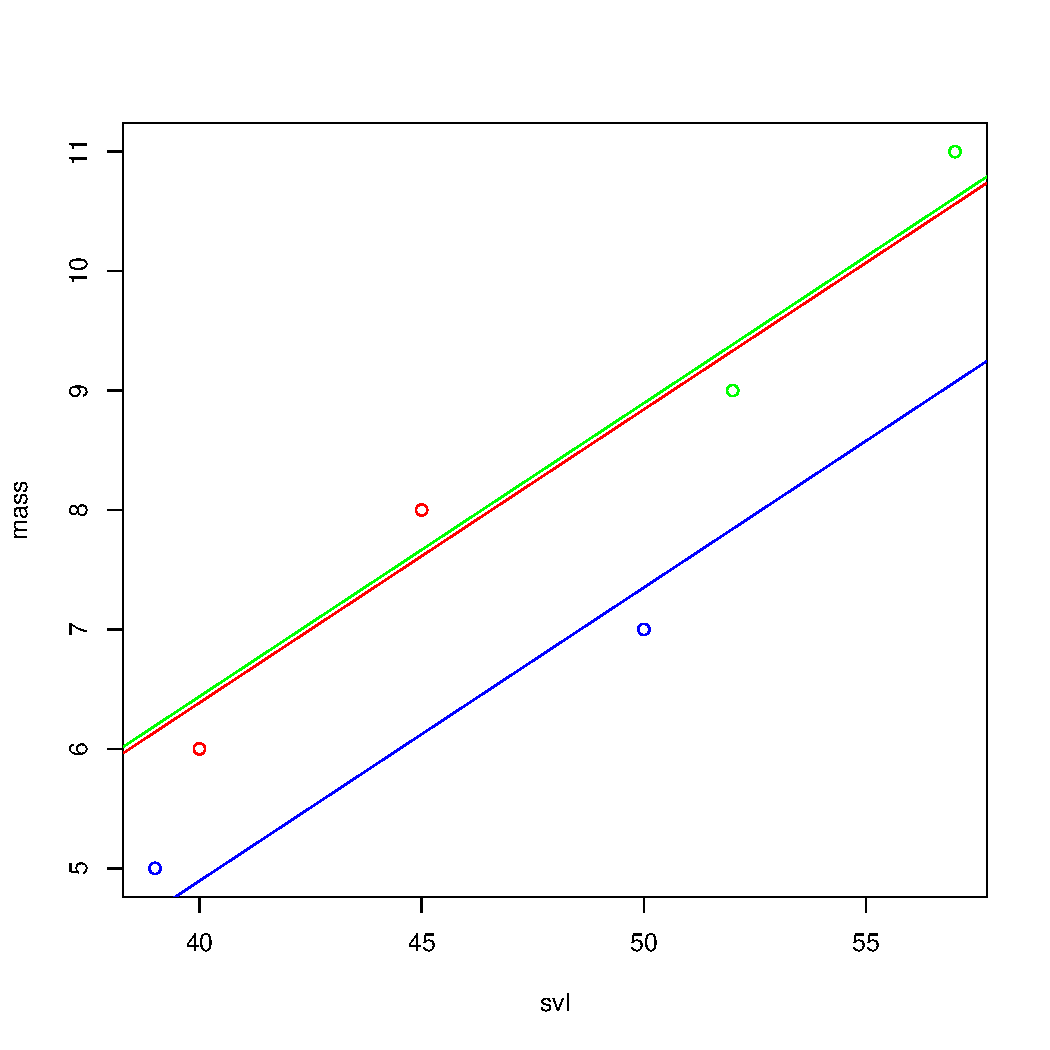
\includegraphics[width=\maxwidth]{figure/unnamed-chunk-111} 
\begin{kframe}\begin{alltt}
\hlcom{# }
\hlstd{fm} \hlkwb{<-} \hlkwd{lm}\hlstd{(mass} \hlopt{~} \hlstd{pop} \hlopt{*} \hlstd{svl)}  \hlcom{# Refit model}
\hlstd{fm}
\end{alltt}
\begin{verbatim}
## 
## Call:
## lm(formula = mass ~ pop * svl)
## 
## Coefficients:
## (Intercept)         pop2         pop3          svl     pop2:svl  
##   -1.00e+01     7.91e+00    -1.80e+00     4.00e-01    -2.18e-01  
##    pop3:svl  
##   -1.60e-15
\end{verbatim}
\begin{alltt}
\hlkwd{model.matrix}\hlstd{(}\hlopt{~}\hlstd{pop} \hlopt{*} \hlstd{svl)}
\end{alltt}
\begin{verbatim}
##   (Intercept) pop2 pop3 svl pop2:svl pop3:svl
## 1           1    0    0  40        0        0
## 2           1    0    0  45        0        0
## 3           1    1    0  39       39        0
## 4           1    1    0  50       50        0
## 5           1    0    1  52        0       52
## 6           1    0    1  57        0       57
## attr(,"assign")
## [1] 0 1 1 2 3 3
## attr(,"contrasts")
## attr(,"contrasts")$pop
## [1] "contr.treatment"
\end{verbatim}
\begin{alltt}
\hlkwd{plot}\hlstd{(svl, mass,} \hlkwc{col} \hlstd{=} \hlkwd{c}\hlstd{(}\hlkwd{rep}\hlstd{(}\hlstr{"red"}\hlstd{,} \hlnum{2}\hlstd{),} \hlkwd{rep}\hlstd{(}\hlstr{"blue"}\hlstd{,} \hlnum{2}\hlstd{),} \hlkwd{rep}\hlstd{(}\hlstr{"green"}\hlstd{,} \hlnum{2}\hlstd{)))}
\hlkwd{abline}\hlstd{(fm}\hlopt{$}\hlstd{coef[}\hlnum{1}\hlstd{], fm}\hlopt{$}\hlstd{coef[}\hlnum{4}\hlstd{],} \hlkwc{col} \hlstd{=} \hlstr{"red"}\hlstd{)}
\hlkwd{abline}\hlstd{(fm}\hlopt{$}\hlstd{coef[}\hlnum{1}\hlstd{]} \hlopt{+} \hlstd{fm}\hlopt{$}\hlstd{coef[}\hlnum{2}\hlstd{], fm}\hlopt{$}\hlstd{coef[}\hlnum{4}\hlstd{]} \hlopt{+} \hlstd{fm}\hlopt{$}\hlstd{coef[}\hlnum{5}\hlstd{],} \hlkwc{col} \hlstd{=} \hlstr{"blue"}\hlstd{)}
\hlkwd{abline}\hlstd{(fm}\hlopt{$}\hlstd{coef[}\hlnum{1}\hlstd{]} \hlopt{+} \hlstd{fm}\hlopt{$}\hlstd{coef[}\hlnum{3}\hlstd{], fm}\hlopt{$}\hlstd{coef[}\hlnum{4}\hlstd{]} \hlopt{+} \hlstd{fm}\hlopt{$}\hlstd{coef[}\hlnum{6}\hlstd{],} \hlkwc{col} \hlstd{=} \hlstr{"green"}\hlstd{)}
\end{alltt}
\end{kframe}
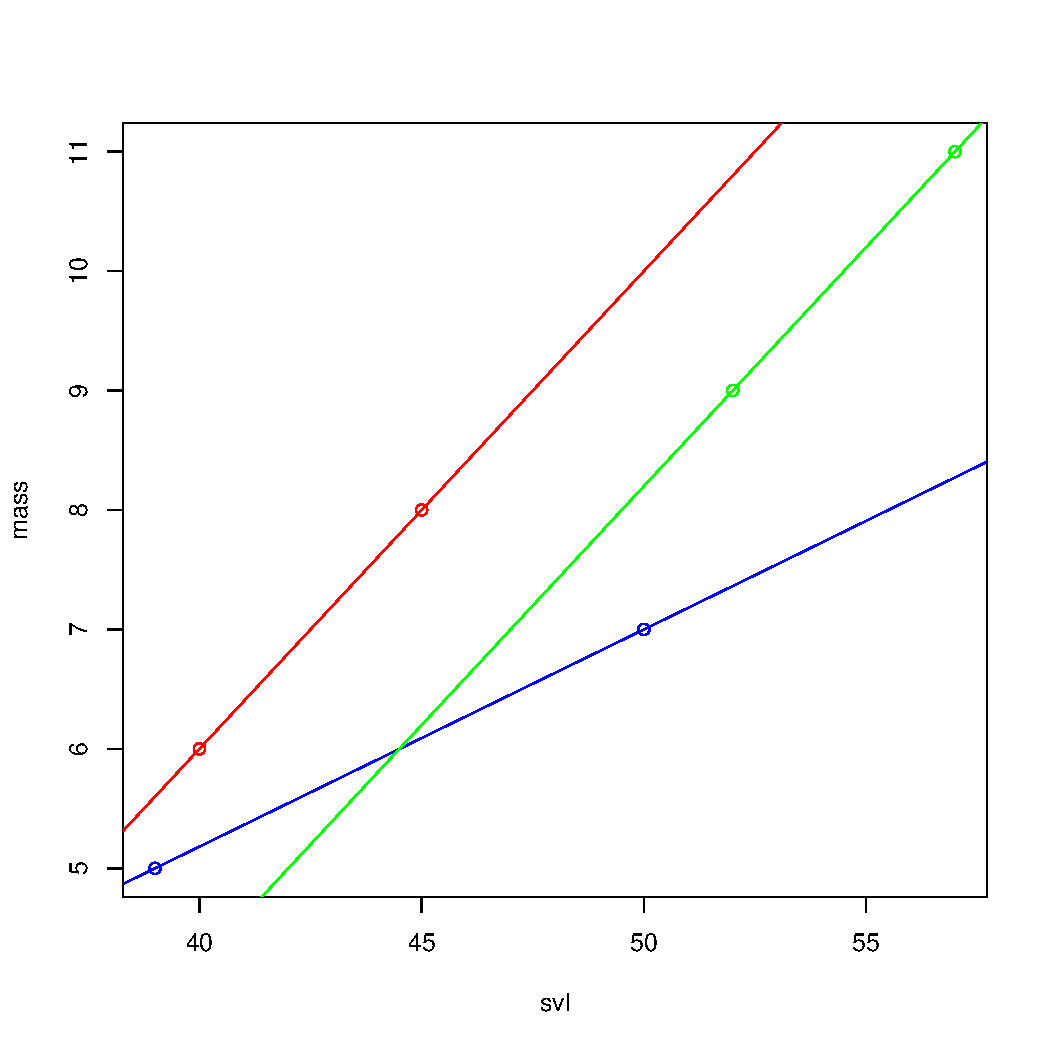
\includegraphics[width=\maxwidth]{figure/unnamed-chunk-112} 
\begin{kframe}\begin{alltt}
\hlcom{# }
\hlstd{fm} \hlkwb{<-} \hlkwd{lm}\hlstd{(mass} \hlopt{~} \hlstd{pop} \hlopt{+} \hlstd{svl} \hlopt{-} \hlnum{1}\hlstd{)}
\hlstd{fm}
\end{alltt}
\begin{verbatim}
## 
## Call:
## lm(formula = mass ~ pop + svl - 1)
## 
## Coefficients:
##   pop1    pop2    pop3     svl  
## -3.439  -4.930  -3.386   0.246
\end{verbatim}
\begin{alltt}
\hlkwd{model.matrix}\hlstd{(}\hlopt{~}\hlstd{pop} \hlopt{+} \hlstd{svl} \hlopt{-} \hlnum{1}\hlstd{)}
\end{alltt}
\begin{verbatim}
##   pop1 pop2 pop3 svl
## 1    1    0    0  40
## 2    1    0    0  45
## 3    0    1    0  39
## 4    0    1    0  50
## 5    0    0    1  52
## 6    0    0    1  57
## attr(,"assign")
## [1] 1 1 1 2
## attr(,"contrasts")
## attr(,"contrasts")$pop
## [1] "contr.treatment"
\end{verbatim}
\begin{alltt}
\hlkwd{plot}\hlstd{(svl, mass,} \hlkwc{col} \hlstd{=} \hlkwd{c}\hlstd{(}\hlkwd{rep}\hlstd{(}\hlstr{"red"}\hlstd{,} \hlnum{2}\hlstd{),} \hlkwd{rep}\hlstd{(}\hlstr{"blue"}\hlstd{,} \hlnum{2}\hlstd{),} \hlkwd{rep}\hlstd{(}\hlstr{"green"}\hlstd{,} \hlnum{2}\hlstd{)))}
\hlkwd{abline}\hlstd{(fm}\hlopt{$}\hlstd{coef[}\hlnum{1}\hlstd{], fm}\hlopt{$}\hlstd{coef[}\hlnum{4}\hlstd{],} \hlkwc{col} \hlstd{=} \hlstr{"red"}\hlstd{)}
\hlkwd{abline}\hlstd{(fm}\hlopt{$}\hlstd{coef[}\hlnum{2}\hlstd{], fm}\hlopt{$}\hlstd{coef[}\hlnum{4}\hlstd{],} \hlkwc{col} \hlstd{=} \hlstr{"blue"}\hlstd{)}
\hlkwd{abline}\hlstd{(fm}\hlopt{$}\hlstd{coef[}\hlnum{3}\hlstd{], fm}\hlopt{$}\hlstd{coef[}\hlnum{4}\hlstd{],} \hlkwc{col} \hlstd{=} \hlstr{"green"}\hlstd{)}
\end{alltt}
\end{kframe}
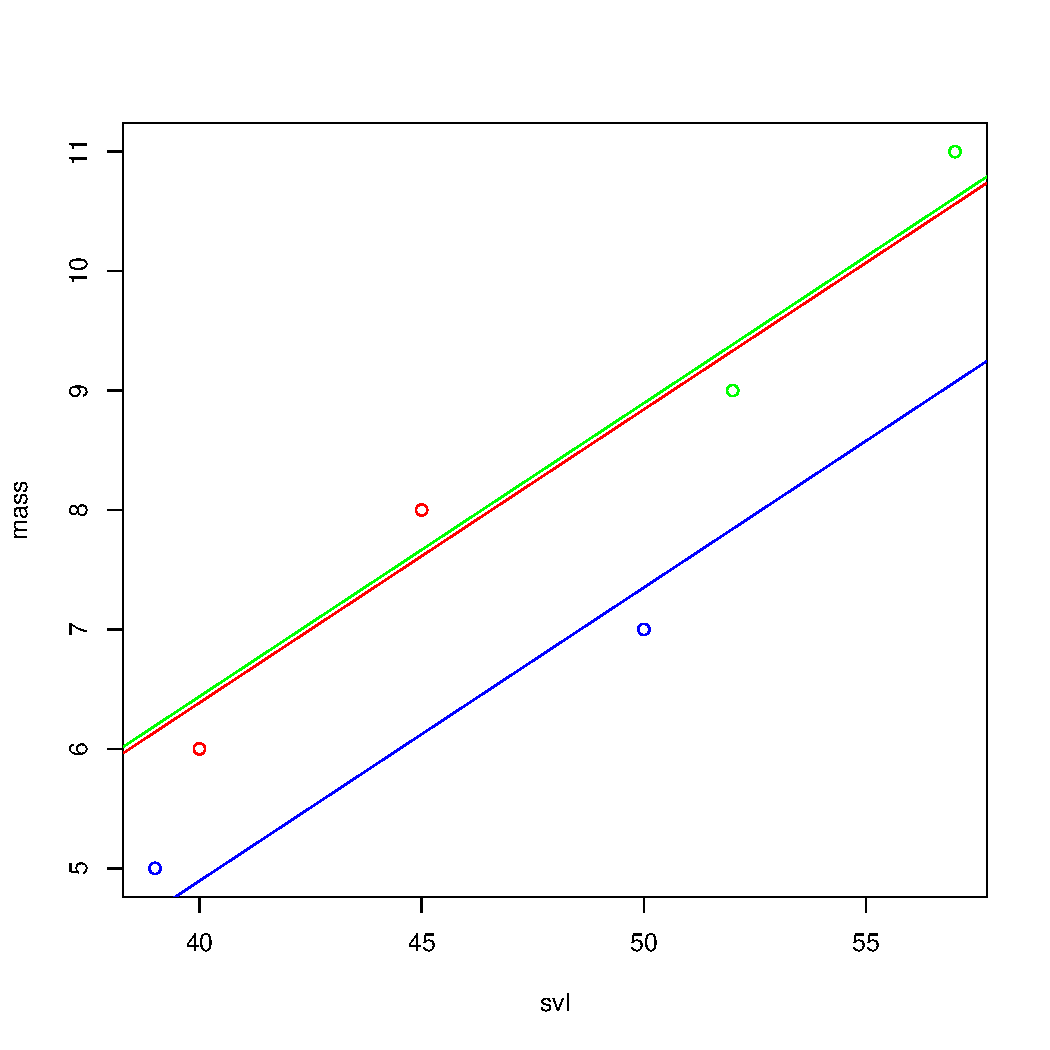
\includegraphics[width=\maxwidth]{figure/unnamed-chunk-113} 
\begin{kframe}\begin{alltt}
\hlcom{# }
\hlstd{fm} \hlkwb{<-} \hlkwd{lm}\hlstd{(mass} \hlopt{~} \hlstd{pop} \hlopt{*} \hlstd{svl} \hlopt{-} \hlnum{1} \hlopt{-} \hlstd{svl)}
\hlstd{fm}
\end{alltt}
\begin{verbatim}
## 
## Call:
## lm(formula = mass ~ pop * svl - 1 - svl)
## 
## Coefficients:
##     pop1      pop2      pop3  pop1:svl  pop2:svl  pop3:svl  
##  -10.000    -2.091   -11.800     0.400     0.182     0.400
\end{verbatim}
\begin{alltt}
\hlkwd{model.matrix}\hlstd{(}\hlopt{~}\hlstd{pop} \hlopt{*} \hlstd{svl} \hlopt{-} \hlnum{1} \hlopt{-} \hlstd{svl)}
\end{alltt}
\begin{verbatim}
##   pop1 pop2 pop3 pop1:svl pop2:svl pop3:svl
## 1    1    0    0       40        0        0
## 2    1    0    0       45        0        0
## 3    0    1    0        0       39        0
## 4    0    1    0        0       50        0
## 5    0    0    1        0        0       52
## 6    0    0    1        0        0       57
## attr(,"assign")
## [1] 1 1 1 2 2 2
## attr(,"contrasts")
## attr(,"contrasts")$pop
## [1] "contr.treatment"
\end{verbatim}
\begin{alltt}
\hlkwd{plot}\hlstd{(svl, mass,} \hlkwc{col} \hlstd{=} \hlkwd{c}\hlstd{(}\hlkwd{rep}\hlstd{(}\hlstr{"red"}\hlstd{,} \hlnum{2}\hlstd{),} \hlkwd{rep}\hlstd{(}\hlstr{"blue"}\hlstd{,} \hlnum{2}\hlstd{),} \hlkwd{rep}\hlstd{(}\hlstr{"green"}\hlstd{,} \hlnum{2}\hlstd{)))}
\hlkwd{abline}\hlstd{(fm}\hlopt{$}\hlstd{coef[}\hlnum{1}\hlstd{], fm}\hlopt{$}\hlstd{coef[}\hlnum{4}\hlstd{],} \hlkwc{col} \hlstd{=} \hlstr{"red"}\hlstd{)}
\hlkwd{abline}\hlstd{(fm}\hlopt{$}\hlstd{coef[}\hlnum{2}\hlstd{], fm}\hlopt{$}\hlstd{coef[}\hlnum{5}\hlstd{],} \hlkwc{col} \hlstd{=} \hlstr{"blue"}\hlstd{)}
\hlkwd{abline}\hlstd{(fm}\hlopt{$}\hlstd{coef[}\hlnum{3}\hlstd{], fm}\hlopt{$}\hlstd{coef[}\hlnum{6}\hlstd{],} \hlkwc{col} \hlstd{=} \hlstr{"green"}\hlstd{)}
\end{alltt}
\end{kframe}
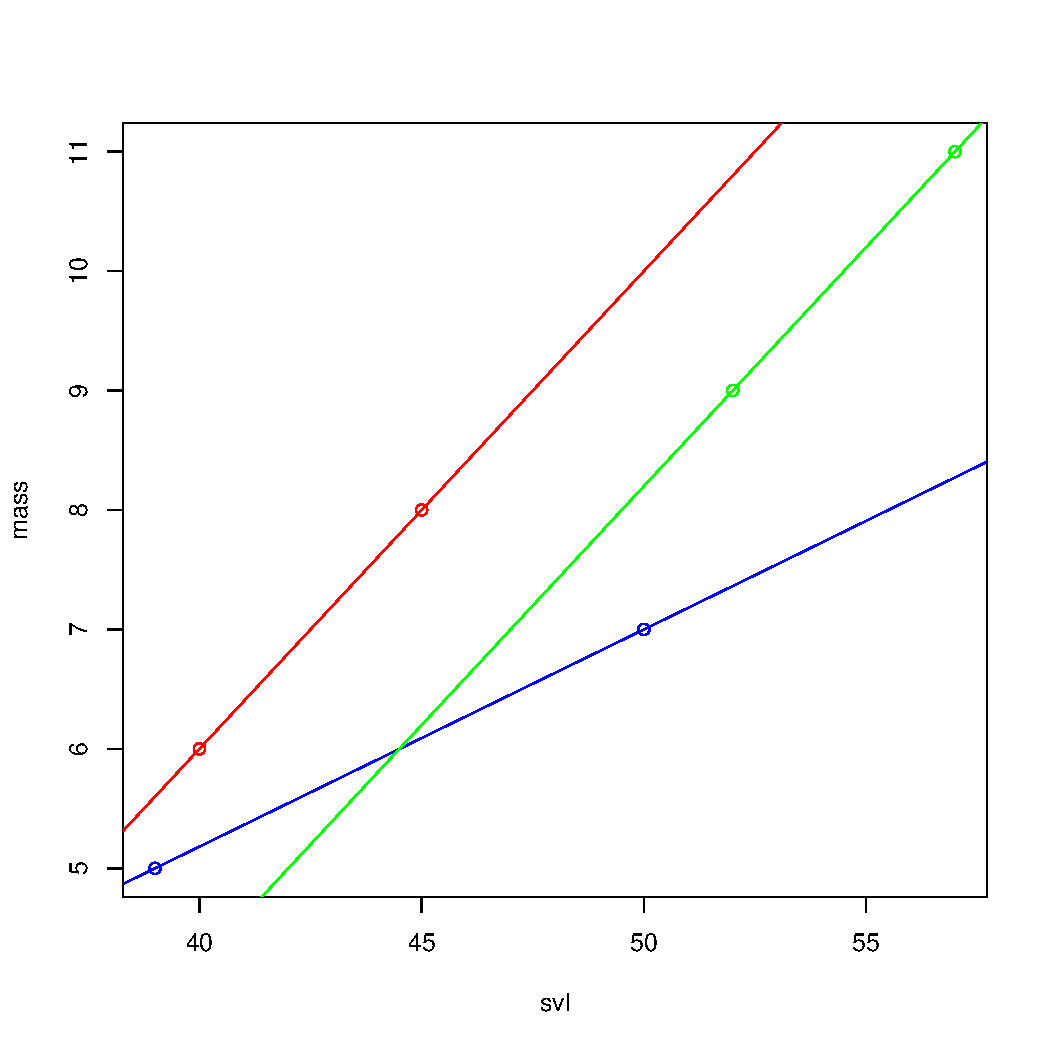
\includegraphics[width=\maxwidth]{figure/unnamed-chunk-114} 

\end{knitrout}




第三章  真正的T检验
\begin{knitrout}
\definecolor{shadecolor}{rgb}{0.969, 0.969, 0.969}\color{fgcolor}\begin{kframe}
\begin{alltt}
\hlcom{# data ~~~~~~~~~~~~~~~~~~}
\hlstd{n1} \hlkwb{<-} \hlnum{60}  \hlcom{# Number of females}
\hlstd{n2} \hlkwb{<-} \hlnum{40}  \hlcom{# Number of males}
\hlstd{mu1} \hlkwb{<-} \hlnum{105}  \hlcom{# Population mean of females}
\hlstd{mu2} \hlkwb{<-} \hlnum{77.5}  \hlcom{# Population mean of males}
\hlstd{sigma} \hlkwb{<-} \hlnum{2.75}  \hlcom{# Average population SD of both}
\hlstd{n} \hlkwb{<-} \hlstd{n1} \hlopt{+} \hlstd{n2}  \hlcom{# Total sample size}
\hlcom{# }
\hlstd{y1} \hlkwb{<-} \hlkwd{rnorm}\hlstd{(n1, mu1, sigma)}  \hlcom{# Data for females}
\hlstd{y2} \hlkwb{<-} \hlkwd{rnorm}\hlstd{(n2, mu2, sigma)}  \hlcom{# Date for males}
\hlstd{y} \hlkwb{<-} \hlkwd{c}\hlstd{(y1, y2)}  \hlcom{# Aggregate both data sets}
\hlstd{x} \hlkwb{<-} \hlkwd{rep}\hlstd{(}\hlkwd{c}\hlstd{(}\hlnum{0}\hlstd{,} \hlnum{1}\hlstd{),} \hlkwd{c}\hlstd{(n1, n2))}  \hlcom{# Indicator for male}
\hlkwd{boxplot}\hlstd{(y} \hlopt{~} \hlstd{x,} \hlkwc{col} \hlstd{=} \hlstr{"grey"}\hlstd{,} \hlkwc{xlab} \hlstd{=} \hlstr{"Male"}\hlstd{,} \hlkwc{ylab} \hlstd{=} \hlstr{"Wingspan (cm)"}\hlstd{,} \hlkwc{las} \hlstd{=} \hlnum{1}\hlstd{)}
\end{alltt}
\end{kframe}
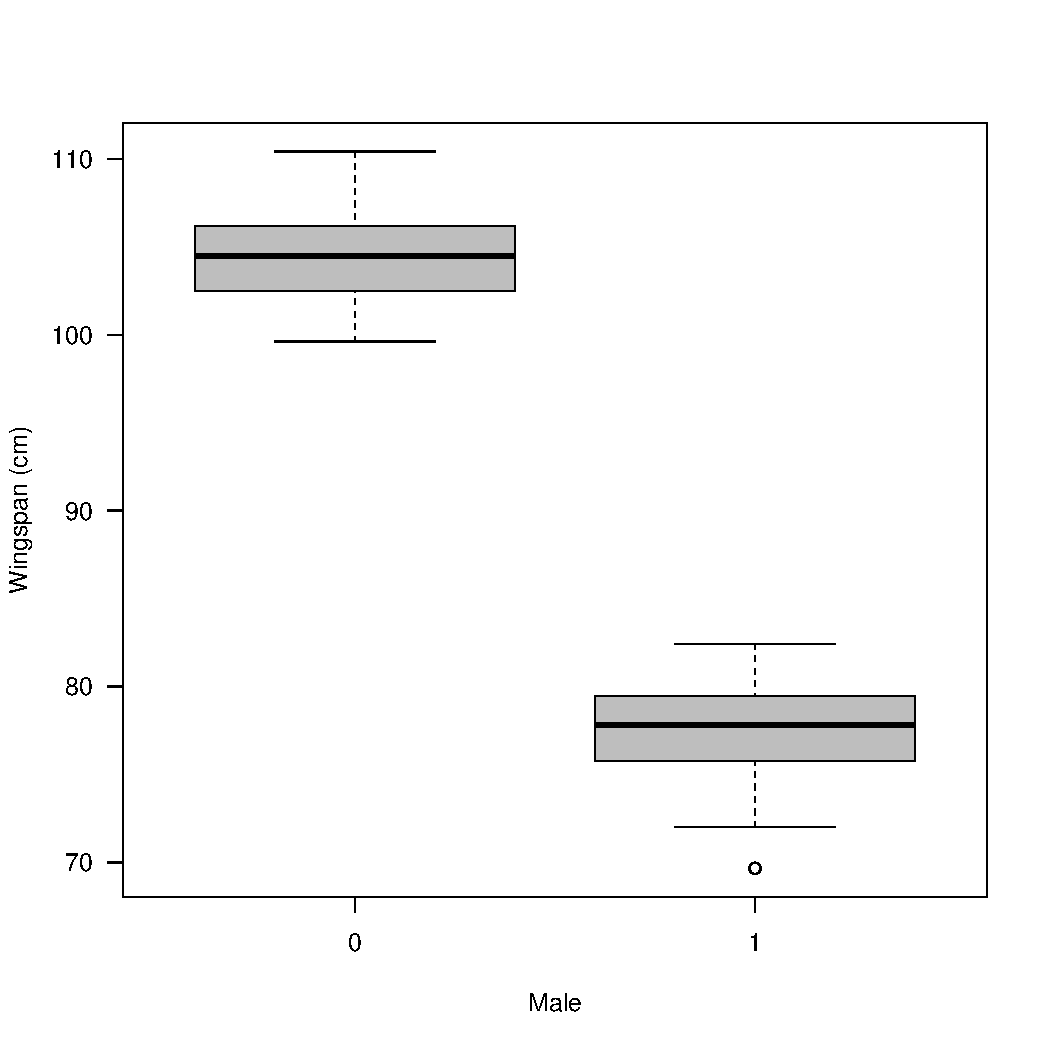
\includegraphics[width=\maxwidth]{figure/unnamed-chunk-121} 
\begin{kframe}\begin{alltt}
\hlcom{# data}
\hlstd{n} \hlkwb{<-} \hlstd{n1} \hlopt{+} \hlstd{n2}  \hlcom{# Total sample size}
\hlstd{alpha} \hlkwb{<-} \hlstd{mu1}  \hlcom{# Mean for females serves as the intercept}
\hlstd{beta} \hlkwb{<-} \hlstd{mu2} \hlopt{-} \hlstd{mu1}  \hlcom{# Beta is the difference male female}
\hlstd{E.y} \hlkwb{<-} \hlstd{alpha} \hlopt{+} \hlstd{beta} \hlopt{*} \hlstd{x}  \hlcom{# Expectation}
\hlstd{y.obs} \hlkwb{<-} \hlkwd{rnorm}\hlstd{(}\hlkwc{n} \hlstd{= n,} \hlkwc{mean} \hlstd{= E.y,} \hlkwc{sd} \hlstd{= sigma)}  \hlcom{# Add random variation}
\hlkwd{boxplot}\hlstd{(y.obs} \hlopt{~} \hlstd{x,} \hlkwc{col} \hlstd{=} \hlstr{"grey"}\hlstd{,} \hlkwc{xlab} \hlstd{=} \hlstr{"Male"}\hlstd{,} \hlkwc{ylab} \hlstd{=} \hlstr{"Wingspan (cm)"}\hlstd{,} \hlkwc{las} \hlstd{=} \hlnum{1}\hlstd{)}
\end{alltt}
\end{kframe}
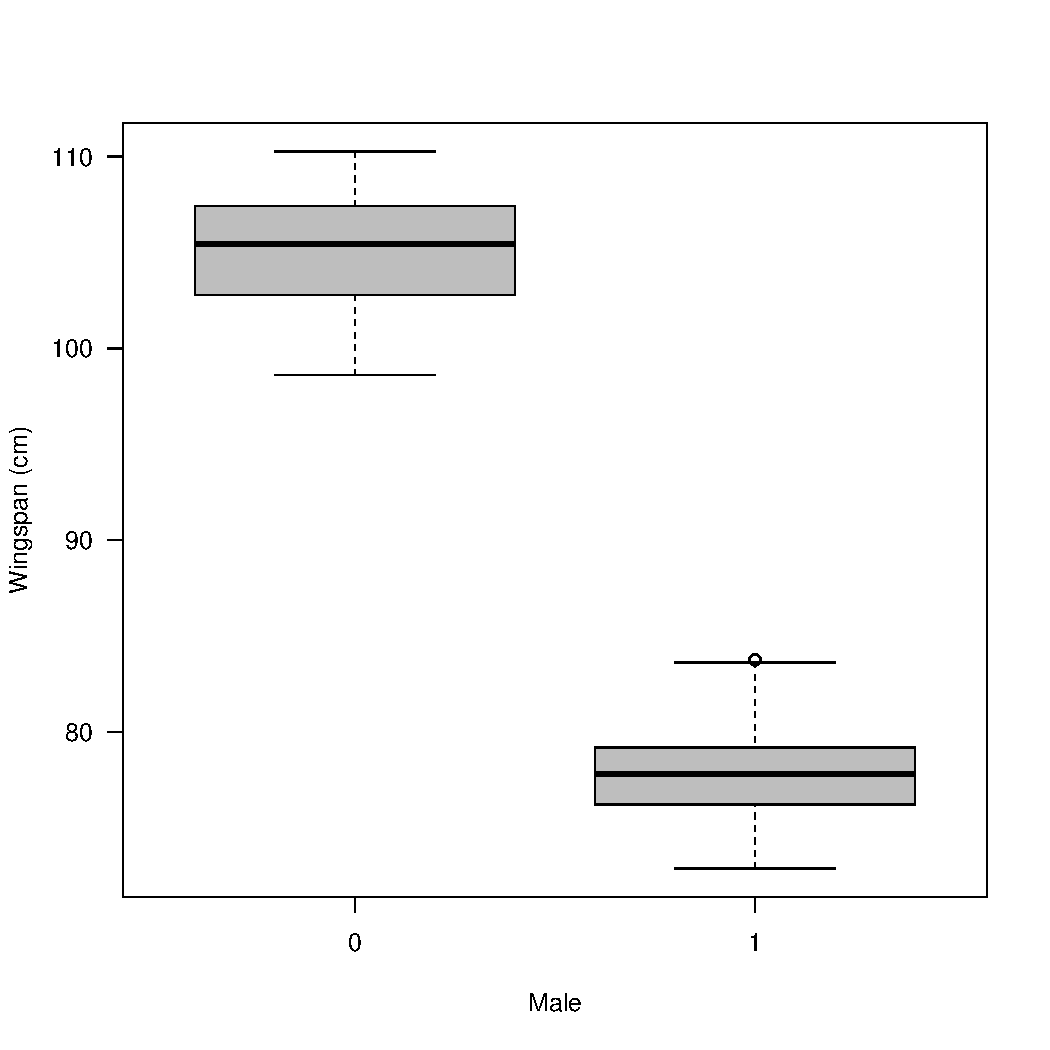
\includegraphics[width=\maxwidth]{figure/unnamed-chunk-122} 
\begin{kframe}\begin{alltt}
\hlcom{# }
\hlstd{fit1} \hlkwb{<-} \hlkwd{lm}\hlstd{(y} \hlopt{~} \hlstd{x)}  \hlcom{# Analysis of first data set}
\hlstd{fit2} \hlkwb{<-} \hlkwd{lm}\hlstd{(y.obs} \hlopt{~} \hlstd{x)}  \hlcom{# Analysis of second data set}
\hlkwd{summary}\hlstd{(fit1)}
\end{alltt}
\begin{verbatim}
## 
## Call:
## lm(formula = y ~ x)
## 
## Residuals:
##    Min     1Q Median     3Q    Max 
## -7.839 -1.813  0.269  1.845  6.035 
## 
## Coefficients:
##             Estimate Std. Error t value Pr(>|t|)    
## (Intercept)  104.387      0.348   300.0   <2e-16 ***
## x            -26.892      0.550   -48.9   <2e-16 ***
## ---
## Signif. codes:  0 '***' 0.001 '**' 0.01 '*' 0.05 '.' 0.1 ' ' 1
## 
## Residual standard error: 2.69 on 98 degrees of freedom
## Multiple R-squared:  0.961,	Adjusted R-squared:  0.96 
## F-statistic: 2.39e+03 on 1 and 98 DF,  p-value: <2e-16
\end{verbatim}
\begin{alltt}
\hlkwd{summary}\hlstd{(fit2)}
\end{alltt}
\begin{verbatim}
## 
## Call:
## lm(formula = y.obs ~ x)
## 
## Residuals:
##    Min     1Q Median     3Q    Max 
## -6.473 -2.001  0.137  1.973  5.977 
## 
## Coefficients:
##             Estimate Std. Error t value Pr(>|t|)    
## (Intercept)  105.087      0.358   293.6   <2e-16 ***
## x            -27.307      0.566   -48.3   <2e-16 ***
## ---
## Signif. codes:  0 '***' 0.001 '**' 0.01 '*' 0.05 '.' 0.1 ' ' 1
## 
## Residual standard error: 2.77 on 98 degrees of freedom
## Multiple R-squared:  0.96,	Adjusted R-squared:  0.959 
## F-statistic: 2.33e+03 on 1 and 98 DF,  p-value: <2e-16
\end{verbatim}
\begin{alltt}
\hlcom{# }
\hlkwd{anova}\hlstd{(fit1)}
\end{alltt}
\begin{verbatim}
## Analysis of Variance Table
## 
## Response: y
##           Df Sum Sq Mean Sq F value Pr(>F)    
## x          1  17357   17357    2390 <2e-16 ***
## Residuals 98    712       7                   
## ---
## Signif. codes:  0 '***' 0.001 '**' 0.01 '*' 0.05 '.' 0.1 ' ' 1
\end{verbatim}
\begin{alltt}
\hlkwd{anova}\hlstd{(fit2)}
\end{alltt}
\begin{verbatim}
## Analysis of Variance Table
## 
## Response: y.obs
##           Df Sum Sq Mean Sq F value Pr(>F)    
## x          1  17896   17896    2329 <2e-16 ***
## Residuals 98    753       8                   
## ---
## Signif. codes:  0 '***' 0.001 '**' 0.01 '*' 0.05 '.' 0.1 ' ' 1
\end{verbatim}
\begin{alltt}
\hlcom{# }
\hlkwd{model.matrix}\hlstd{(fit1)}
\end{alltt}
\begin{verbatim}
##     (Intercept) x
## 1             1 0
## 2             1 0
## 3             1 0
## 4             1 0
## 5             1 0
## 6             1 0
## 7             1 0
## 8             1 0
## 9             1 0
## 10            1 0
## 11            1 0
## 12            1 0
## 13            1 0
## 14            1 0
## 15            1 0
## 16            1 0
## 17            1 0
## 18            1 0
## 19            1 0
## 20            1 0
## 21            1 0
## 22            1 0
## 23            1 0
## 24            1 0
## 25            1 0
## 26            1 0
## 27            1 0
## 28            1 0
## 29            1 0
## 30            1 0
## 31            1 0
## 32            1 0
## 33            1 0
## 34            1 0
## 35            1 0
## 36            1 0
## 37            1 0
## 38            1 0
## 39            1 0
## 40            1 0
## 41            1 0
## 42            1 0
## 43            1 0
## 44            1 0
## 45            1 0
## 46            1 0
## 47            1 0
## 48            1 0
## 49            1 0
## 50            1 0
## 51            1 0
## 52            1 0
## 53            1 0
## 54            1 0
## 55            1 0
## 56            1 0
## 57            1 0
## 58            1 0
## 59            1 0
## 60            1 0
## 61            1 1
## 62            1 1
## 63            1 1
## 64            1 1
## 65            1 1
## 66            1 1
## 67            1 1
## 68            1 1
## 69            1 1
## 70            1 1
## 71            1 1
## 72            1 1
## 73            1 1
## 74            1 1
## 75            1 1
## 76            1 1
## 77            1 1
## 78            1 1
## 79            1 1
## 80            1 1
## 81            1 1
## 82            1 1
## 83            1 1
## 84            1 1
## 85            1 1
## 86            1 1
## 87            1 1
## 88            1 1
## 89            1 1
## 90            1 1
## 91            1 1
## 92            1 1
## 93            1 1
## 94            1 1
## 95            1 1
## 96            1 1
## 97            1 1
## 98            1 1
## 99            1 1
## 100           1 1
## attr(,"assign")
## [1] 0 1
\end{verbatim}
\begin{alltt}
\hlkwd{model.matrix}\hlstd{(fit2)}
\end{alltt}
\begin{verbatim}
##     (Intercept) x
## 1             1 0
## 2             1 0
## 3             1 0
## 4             1 0
## 5             1 0
## 6             1 0
## 7             1 0
## 8             1 0
## 9             1 0
## 10            1 0
## 11            1 0
## 12            1 0
## 13            1 0
## 14            1 0
## 15            1 0
## 16            1 0
## 17            1 0
## 18            1 0
## 19            1 0
## 20            1 0
## 21            1 0
## 22            1 0
## 23            1 0
## 24            1 0
## 25            1 0
## 26            1 0
## 27            1 0
## 28            1 0
## 29            1 0
## 30            1 0
## 31            1 0
## 32            1 0
## 33            1 0
## 34            1 0
## 35            1 0
## 36            1 0
## 37            1 0
## 38            1 0
## 39            1 0
## 40            1 0
## 41            1 0
## 42            1 0
## 43            1 0
## 44            1 0
## 45            1 0
## 46            1 0
## 47            1 0
## 48            1 0
## 49            1 0
## 50            1 0
## 51            1 0
## 52            1 0
## 53            1 0
## 54            1 0
## 55            1 0
## 56            1 0
## 57            1 0
## 58            1 0
## 59            1 0
## 60            1 0
## 61            1 1
## 62            1 1
## 63            1 1
## 64            1 1
## 65            1 1
## 66            1 1
## 67            1 1
## 68            1 1
## 69            1 1
## 70            1 1
## 71            1 1
## 72            1 1
## 73            1 1
## 74            1 1
## 75            1 1
## 76            1 1
## 77            1 1
## 78            1 1
## 79            1 1
## 80            1 1
## 81            1 1
## 82            1 1
## 83            1 1
## 84            1 1
## 85            1 1
## 86            1 1
## 87            1 1
## 88            1 1
## 89            1 1
## 90            1 1
## 91            1 1
## 92            1 1
## 93            1 1
## 94            1 1
## 95            1 1
## 96            1 1
## 97            1 1
## 98            1 1
## 99            1 1
## 100           1 1
## attr(,"assign")
## [1] 0 1
\end{verbatim}
\end{kframe}
\end{knitrout}




现在来看一下怎么使用bayesian方法实现呢?



\begin{knitrout}
\definecolor{shadecolor}{rgb}{0.969, 0.969, 0.969}\color{fgcolor}\begin{kframe}
\begin{alltt}
\hlcom{## 2.2 Data ~~~~~~~~~~~~~~~~~~~}
\hlkwd{require}\hlstd{(LaplacesDemon)}
\hlcom{##################################################### data ~~~~~~~~~~~~~~~~~~}
\hlstd{n1} \hlkwb{<-} \hlnum{600}  \hlcom{# Number of females}
\hlstd{n2} \hlkwb{<-} \hlnum{400}  \hlcom{# Number of males}
\hlstd{mu1} \hlkwb{<-} \hlnum{105}  \hlcom{# Population mean of females}
\hlstd{mu2} \hlkwb{<-} \hlnum{77.5}  \hlcom{# Population mean of males}
\hlstd{sigma} \hlkwb{<-} \hlnum{1.75}  \hlcom{# Average population SD of both}
\hlcom{# }
\hlstd{n} \hlkwb{<-} \hlstd{n1} \hlopt{+} \hlstd{n2}  \hlcom{# Total sample size}
\hlstd{alpha} \hlkwb{<-} \hlstd{mu1}  \hlcom{# Mean for females serves as the intercept}
\hlstd{beta} \hlkwb{<-} \hlstd{mu1} \hlopt{-} \hlstd{mu2}  \hlcom{# Beta is the difference male female}
\hlstd{x} \hlkwb{<-} \hlkwd{rep}\hlstd{(}\hlkwd{c}\hlstd{(}\hlnum{0}\hlstd{,} \hlnum{1}\hlstd{),} \hlkwd{c}\hlstd{(n1, n2))}
\hlstd{E.y} \hlkwb{<-} \hlstd{alpha} \hlopt{+} \hlstd{beta} \hlopt{*} \hlstd{x}  \hlcom{# Expectation}
\hlstd{y.obs} \hlkwb{<-} \hlkwd{rnorm}\hlstd{(}\hlkwc{n} \hlstd{= n,} \hlkwc{mean} \hlstd{= E.y,} \hlkwc{sd} \hlstd{= sigma)}  \hlcom{# Add random variation}
\hlkwd{boxplot}\hlstd{(y.obs} \hlopt{~} \hlstd{x,} \hlkwc{col} \hlstd{=} \hlstr{"grey"}\hlstd{,} \hlkwc{xlab} \hlstd{=} \hlstr{"Male"}\hlstd{,} \hlkwc{ylab} \hlstd{=} \hlstr{"Wingspan (cm)"}\hlstd{,} \hlkwc{las} \hlstd{=} \hlnum{1}\hlstd{)}
\end{alltt}
\end{kframe}
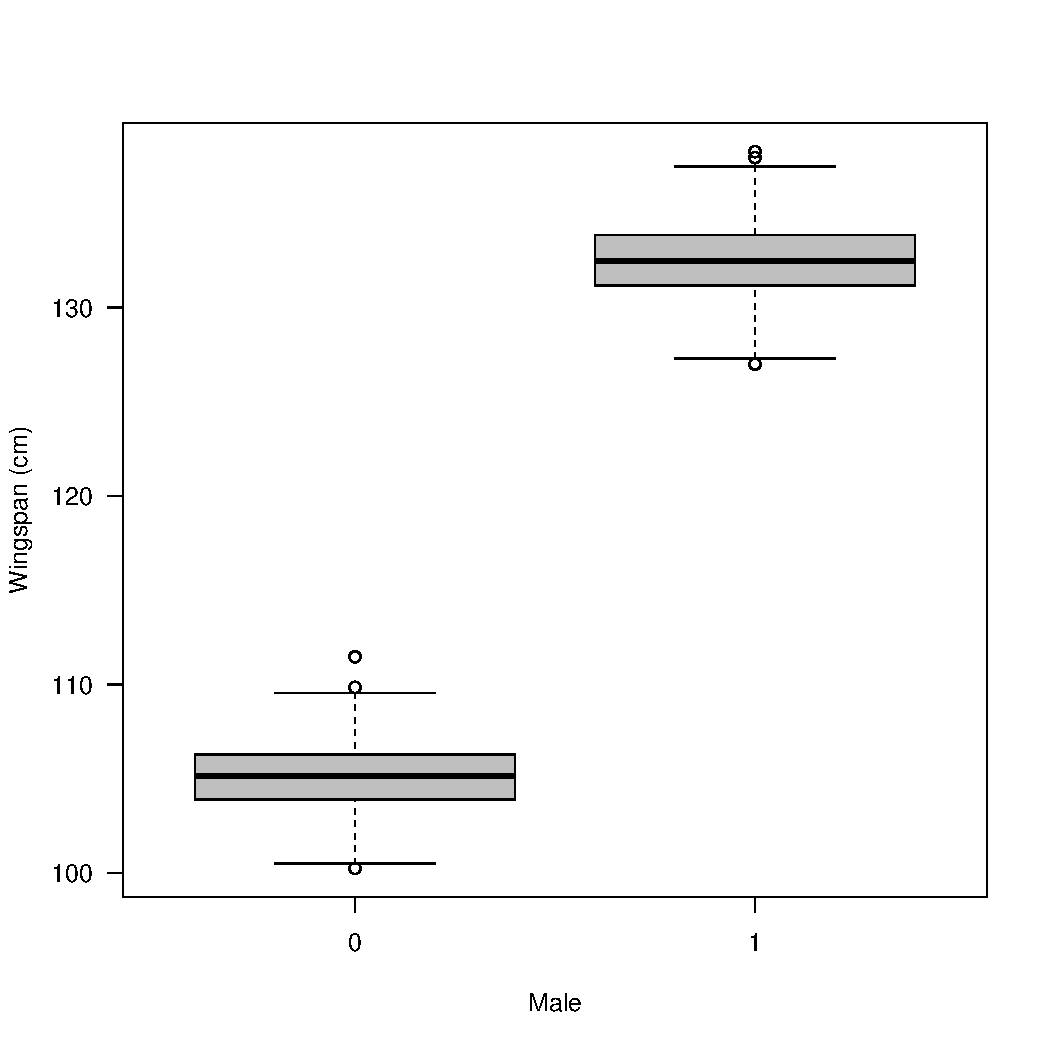
\includegraphics[width=\maxwidth]{figure/unnamed-chunk-131} 
\begin{kframe}\begin{alltt}
\hlcom{###################################################### }
\hlstd{parm.names} \hlkwb{<-} \hlkwd{as.parm.names}\hlstd{(Initial.Values)}
\end{alltt}


{\ttfamily\noindent\bfseries\color{errorcolor}{\#\# Error: replacement has length zero}}\begin{alltt}
\hlstd{mon.names} \hlkwb{<-} \hlkwd{c}\hlstd{(}\hlstr{"LP00"}\hlstd{)}
\hlstd{Data} \hlkwb{<-} \hlstd{MyData} \hlkwb{<-} \hlkwd{list}\hlstd{(}\hlkwc{N} \hlstd{= n,} \hlkwc{mon.names} \hlstd{= mon.names,} \hlkwc{parm.names} \hlstd{= parm.names,}
    \hlkwc{x} \hlstd{= x,} \hlkwc{y} \hlstd{= y.obs)}
\hlcom{## 2.3. Model ~~~~~~~~~~~~~~~~~}
\hlstd{Model} \hlkwb{<-} \hlkwa{function}\hlstd{(}\hlkwc{parm}\hlstd{,} \hlkwc{Data}\hlstd{) \{}
    \hlcom{### Parameters}
    \hlstd{alpha} \hlkwb{<-} \hlstd{parm[}\hlnum{1}\hlstd{]}
    \hlstd{beta} \hlkwb{<-} \hlstd{parm[}\hlnum{2}\hlstd{]}
    \hlstd{sigma} \hlkwb{<-} \hlstd{parm[}\hlnum{3}\hlstd{]}
    \hlcom{### Log(Prior Densities)}
    \hlstd{alpha.prior} \hlkwb{<-} \hlkwd{dnormv}\hlstd{(}\hlkwc{x} \hlstd{= alpha,} \hlkwc{mean} \hlstd{=} \hlnum{0}\hlstd{,} \hlkwc{var} \hlstd{=} \hlnum{1000}\hlstd{,} \hlkwc{log} \hlstd{=} \hlnum{TRUE}\hlstd{)}
    \hlstd{beta.prior} \hlkwb{<-} \hlkwd{dnorm}\hlstd{(}\hlkwc{x} \hlstd{= beta,} \hlkwc{mean} \hlstd{=} \hlnum{0}\hlstd{,} \hlkwc{sd} \hlstd{= sigma,} \hlkwc{log} \hlstd{=} \hlnum{TRUE}\hlstd{)}
    \hlstd{sigma.prior} \hlkwb{<-} \hlkwd{dhalfcauchy}\hlstd{(}\hlkwc{x} \hlstd{= sigma,} \hlkwc{scale} \hlstd{=} \hlnum{25}\hlstd{,} \hlkwc{log} \hlstd{=} \hlnum{TRUE}\hlstd{)}
    \hlcom{### Log-Likelihood}
    \hlstd{mu} \hlkwb{<-} \hlstd{alpha} \hlopt{+} \hlstd{beta} \hlopt{*} \hlstd{Data}\hlopt{$}\hlstd{x}
    \hlstd{LL} \hlkwb{<-} \hlkwd{sum}\hlstd{(}\hlkwd{dnorm}\hlstd{(}\hlkwc{x} \hlstd{= Data}\hlopt{$}\hlstd{y,} \hlkwc{mean} \hlstd{= mu,} \hlkwc{sd} \hlstd{= sigma,} \hlkwc{log} \hlstd{=} \hlnum{TRUE}\hlstd{))}
    \hlcom{### Log-Posterior}
    \hlstd{LP} \hlkwb{<-} \hlstd{LL} \hlopt{+} \hlstd{alpha.prior} \hlopt{+} \hlstd{beta.prior} \hlopt{+} \hlstd{sigma.prior}
    \hlstd{Modelout} \hlkwb{<-} \hlkwd{list}\hlstd{(}\hlkwc{LP} \hlstd{= LP,} \hlkwc{Dev} \hlstd{=} \hlopt{-}\hlnum{2} \hlopt{*} \hlstd{LL,} \hlkwc{Monitor} \hlstd{=} \hlkwd{c}\hlstd{(LP),} \hlkwc{yhat} \hlstd{=} \hlkwd{rnorm}\hlstd{(}\hlkwd{length}\hlstd{(mu),}
        \hlstd{mu, sigma),} \hlkwc{parm} \hlstd{= parm)}
    \hlkwd{return}\hlstd{(Modelout)}
\hlstd{\}}
\hlcom{## 2.4. Initial Values~~~~~~~~~~~~~~}
\hlstd{parm} \hlkwb{<-} \hlstd{Initial.Values} \hlkwb{<-} \hlkwd{c}\hlstd{(}\hlkwc{alpha_11} \hlstd{=} \hlnum{100}\hlstd{,} \hlkwc{beta_11} \hlstd{=} \hlnum{20}\hlstd{,} \hlkwc{sigma_11} \hlstd{=} \hlnum{1}\hlstd{)}
\hlcom{## 2.5 MCMC ~~~~~~~~~~~~~~~~~~~~~~~~~~~~~~~~ MCMC settings}
\hlstd{ni} \hlkwb{<-} \hlnum{10000}  \hlcom{# Number of draws from posterior (for each chain)}
\hlstd{st} \hlkwb{<-} \hlnum{4000}  \hlcom{# Steps when status message should be given}
\hlstd{nt} \hlkwb{<-} \hlnum{50}  \hlcom{# Thinning rate #  Abate autocorrelation}
\hlcom{# Run LaplacesDemon}
\hlstd{out} \hlkwb{<-} \hlkwd{LaplacesDemon}\hlstd{(Model,} \hlkwc{Data} \hlstd{= MyData, Initial.Values,} \hlkwc{Iterations} \hlstd{= ni,}
    \hlkwc{Status} \hlstd{= st,} \hlkwc{Thinning} \hlstd{= nt)}
\end{alltt}
\begin{verbatim}
## 
## Laplace's Demon was called on Wed Oct 30 18:04:59 2013
## 
## Performing initial checks...
## WARNING: The length of Initial Values differed from Data$parm.names.
\end{verbatim}


{\ttfamily\noindent\color{warningcolor}{\#\# Warning: NAs produced}}\begin{verbatim}
## Generating initial values due to a non-finite posterior.
\end{verbatim}


{\ttfamily\noindent\color{warningcolor}{\#\# Warning: NAs produced\\\#\# Warning: NAs produced\\\#\# Warning: NAs produced\\\#\# Warning: NAs produced\\\#\# Warning: NAs produced\\\#\# Warning: NAs produced\\\#\# Warning: NAs produced\\\#\# Warning: NAs produced\\\#\# Warning: NAs produced\\\#\# Warning: NAs produced\\\#\# Warning: NAs produced\\\#\# Warning: NAs produced\\\#\# Warning: NAs produced\\\#\# Warning: NAs produced\\\#\# Warning: NAs produced\\\#\# Warning: NAs produced\\\#\# Warning: NAs produced\\\#\# Warning: NAs produced\\\#\# Warning: NAs produced\\\#\# Warning: NAs produced\\\#\# Warning: NAs produced\\\#\# Warning: NAs produced\\\#\# Warning: NAs produced\\\#\# Warning: NAs produced\\\#\# Warning: NAs produced\\\#\# Warning: NAs produced\\\#\# Warning: NAs produced\\\#\# Warning: NAs produced\\\#\# Warning: NAs produced\\\#\# Warning: NAs produced\\\#\# Warning: NAs produced\\\#\# Warning: NAs produced\\\#\# Warning: NAs produced\\\#\# Warning: NAs produced\\\#\# Warning: NAs produced\\\#\# Warning: NAs produced\\\#\# Warning: NAs produced\\\#\# Warning: NAs produced\\\#\# Warning: NAs produced\\\#\# Warning: NAs produced\\\#\# Warning: NAs produced\\\#\# Warning: NAs produced\\\#\# Warning: NAs produced\\\#\# Warning: NAs produced\\\#\# Warning: NAs produced\\\#\# Warning: NAs produced\\\#\# Warning: NAs produced\\\#\# Warning: NAs produced\\\#\# Warning: NAs produced\\\#\# Warning: NAs produced\\\#\# Warning: NAs produced\\\#\# Warning: NAs produced\\\#\# Warning: NAs produced\\\#\# Warning: NAs produced\\\#\# Warning: NAs produced\\\#\# Warning: NAs produced\\\#\# Warning: NAs produced\\\#\# Warning: NAs produced\\\#\# Warning: NAs produced\\\#\# Warning: NAs produced\\\#\# Warning: NAs produced\\\#\# Warning: NAs produced\\\#\# Warning: NAs produced\\\#\# Warning: NAs produced\\\#\# Warning: NAs produced\\\#\# Warning: NAs produced\\\#\# Warning: NAs produced\\\#\# Warning: NAs produced\\\#\# Warning: NAs produced\\\#\# Warning: NAs produced\\\#\# Warning: NAs produced\\\#\# Warning: NAs produced\\\#\# Warning: NAs produced\\\#\# Warning: NAs produced\\\#\# Warning: NAs produced\\\#\# Warning: NAs produced\\\#\# Warning: NAs produced\\\#\# Warning: NAs produced\\\#\# Warning: NAs produced\\\#\# Warning: NAs produced\\\#\# Warning: NAs produced\\\#\# Warning: NAs produced\\\#\# Warning: NAs produced\\\#\# Warning: NAs produced\\\#\# Warning: NAs produced\\\#\# Warning: NAs produced\\\#\# Warning: NAs produced\\\#\# Warning: NAs produced\\\#\# Warning: NAs produced\\\#\# Warning: NAs produced\\\#\# Warning: NAs produced\\\#\# Warning: NAs produced\\\#\# Warning: NAs produced\\\#\# Warning: NAs produced\\\#\# Warning: NAs produced\\\#\# Warning: NAs produced\\\#\# Warning: NAs produced\\\#\# Warning: NAs produced\\\#\# Warning: NAs produced\\\#\# Warning: NAs produced\\\#\# Warning: NAs produced\\\#\# Warning: NAs produced\\\#\# Warning: NAs produced\\\#\# Warning: NAs produced\\\#\# Warning: NAs produced\\\#\# Warning: NAs produced\\\#\# Warning: NAs produced\\\#\# Warning: NAs produced\\\#\# Warning: NAs produced\\\#\# Warning: NAs produced\\\#\# Warning: NAs produced\\\#\# Warning: NAs produced\\\#\# Warning: NAs produced\\\#\# Warning: NAs produced\\\#\# Warning: NAs produced\\\#\# Warning: NAs produced\\\#\# Warning: NAs produced\\\#\# Warning: NAs produced\\\#\# Warning: NAs produced\\\#\# Warning: NAs produced\\\#\# Warning: NAs produced\\\#\# Warning: NAs produced\\\#\# Warning: NAs produced\\\#\# Warning: NAs produced\\\#\# Warning: NAs produced\\\#\# Warning: NAs produced\\\#\# Warning: NAs produced\\\#\# Warning: NAs produced\\\#\# Warning: NAs produced\\\#\# Warning: NAs produced\\\#\# Warning: NAs produced\\\#\# Warning: NAs produced\\\#\# Warning: NAs produced\\\#\# Warning: NAs produced\\\#\# Warning: NAs produced\\\#\# Warning: NAs produced\\\#\# Warning: NAs produced\\\#\# Warning: NAs produced\\\#\# Warning: NAs produced\\\#\# Warning: NAs produced\\\#\# Warning: NAs produced\\\#\# Warning: NAs produced\\\#\# Warning: NAs produced\\\#\# Warning: NAs produced\\\#\# Warning: NAs produced\\\#\# Warning: NAs produced\\\#\# Warning: NAs produced\\\#\# Warning: NAs produced\\\#\# Warning: NAs produced\\\#\# Warning: NAs produced\\\#\# Warning: NAs produced\\\#\# Warning: NAs produced\\\#\# Warning: NAs produced\\\#\# Warning: NAs produced\\\#\# Warning: NAs produced\\\#\# Warning: NAs produced\\\#\# Warning: NAs produced\\\#\# Warning: NAs produced\\\#\# Warning: NAs produced\\\#\# Warning: NAs produced\\\#\# Warning: NAs produced\\\#\# Warning: NAs produced\\\#\# Warning: NAs produced\\\#\# Warning: NAs produced\\\#\# Warning: NAs produced\\\#\# Warning: NAs produced\\\#\# Warning: NAs produced\\\#\# Warning: NAs produced\\\#\# Warning: NAs produced\\\#\# Warning: NAs produced\\\#\# Warning: NAs produced\\\#\# Warning: NAs produced\\\#\# Warning: NAs produced\\\#\# Warning: NAs produced\\\#\# Warning: NAs produced\\\#\# Warning: NAs produced\\\#\# Warning: NAs produced\\\#\# Warning: NAs produced\\\#\# Warning: NAs produced\\\#\# Warning: NAs produced\\\#\# Warning: NAs produced\\\#\# Warning: NAs produced\\\#\# Warning: NAs produced\\\#\# Warning: NAs produced\\\#\# Warning: NAs produced\\\#\# Warning: NAs produced\\\#\# Warning: NAs produced\\\#\# Warning: NAs produced\\\#\# Warning: NAs produced\\\#\# Warning: NAs produced\\\#\# Warning: NAs produced\\\#\# Warning: NAs produced\\\#\# Warning: NAs produced\\\#\# Warning: NAs produced\\\#\# Warning: NAs produced\\\#\# Warning: NAs produced\\\#\# Warning: NAs produced\\\#\# Warning: NAs produced\\\#\# Warning: NAs produced\\\#\# Warning: NAs produced\\\#\# Warning: NAs produced\\\#\# Warning: NAs produced\\\#\# Warning: NAs produced\\\#\# Warning: NAs produced\\\#\# Warning: NAs produced\\\#\# Warning: NAs produced\\\#\# Warning: NAs produced\\\#\# Warning: NAs produced\\\#\# Warning: NAs produced\\\#\# Warning: NAs produced\\\#\# Warning: NAs produced\\\#\# Warning: NAs produced\\\#\# Warning: NAs produced\\\#\# Warning: NAs produced\\\#\# Warning: NAs produced\\\#\# Warning: NAs produced\\\#\# Warning: NAs produced\\\#\# Warning: NAs produced\\\#\# Warning: NAs produced\\\#\# Warning: NAs produced\\\#\# Warning: NAs produced\\\#\# Warning: NAs produced\\\#\# Warning: NAs produced\\\#\# Warning: NAs produced\\\#\# Warning: NAs produced\\\#\# Warning: NAs produced\\\#\# Warning: NAs produced\\\#\# Warning: NAs produced\\\#\# Warning: NAs produced\\\#\# Warning: NAs produced\\\#\# Warning: NAs produced\\\#\# Warning: NAs produced\\\#\# Warning: NAs produced\\\#\# Warning: NAs produced\\\#\# Warning: NAs produced\\\#\# Warning: NAs produced\\\#\# Warning: NAs produced\\\#\# Warning: NAs produced\\\#\# Warning: NAs produced\\\#\# Warning: NAs produced\\\#\# Warning: NAs produced\\\#\# Warning: NAs produced\\\#\# Warning: NAs produced\\\#\# Warning: NAs produced\\\#\# Warning: NAs produced\\\#\# Warning: NAs produced\\\#\# Warning: NAs produced\\\#\# Warning: NAs produced\\\#\# Warning: NAs produced\\\#\# Warning: NAs produced\\\#\# Warning: NAs produced\\\#\# Warning: NAs produced\\\#\# Warning: NAs produced\\\#\# Warning: NAs produced\\\#\# Warning: NAs produced\\\#\# Warning: NAs produced\\\#\# Warning: NAs produced\\\#\# Warning: NAs produced\\\#\# Warning: NAs produced\\\#\# Warning: NAs produced\\\#\# Warning: NAs produced\\\#\# Warning: NAs produced\\\#\# Warning: NAs produced\\\#\# Warning: NAs produced\\\#\# Warning: NAs produced\\\#\# Warning: NAs produced\\\#\# Warning: NAs produced\\\#\# Warning: NAs produced\\\#\# Warning: NAs produced\\\#\# Warning: NAs produced\\\#\# Warning: NAs produced\\\#\# Warning: NAs produced\\\#\# Warning: NAs produced\\\#\# Warning: NAs produced\\\#\# Warning: NAs produced\\\#\# Warning: NAs produced\\\#\# Warning: NAs produced\\\#\# Warning: NAs produced\\\#\# Warning: NAs produced\\\#\# Warning: NAs produced\\\#\# Warning: NAs produced\\\#\# Warning: NAs produced\\\#\# Warning: NAs produced\\\#\# Warning: NAs produced\\\#\# Warning: NAs produced\\\#\# Warning: NAs produced\\\#\# Warning: NAs produced\\\#\# Warning: NAs produced\\\#\# Warning: NAs produced\\\#\# Warning: NAs produced\\\#\# Warning: NAs produced\\\#\# Warning: NAs produced\\\#\# Warning: NAs produced\\\#\# Warning: NAs produced\\\#\# Warning: NAs produced\\\#\# Warning: NAs produced\\\#\# Warning: NAs produced\\\#\# Warning: NAs produced\\\#\# Warning: NAs produced\\\#\# Warning: NAs produced\\\#\# Warning: NAs produced\\\#\# Warning: NAs produced\\\#\# Warning: NAs produced\\\#\# Warning: NAs produced\\\#\# Warning: NAs produced\\\#\# Warning: NAs produced\\\#\# Warning: NAs produced\\\#\# Warning: NAs produced\\\#\# Warning: NAs produced\\\#\# Warning: NAs produced\\\#\# Warning: NAs produced\\\#\# Warning: NAs produced\\\#\# Warning: NAs produced\\\#\# Warning: NAs produced\\\#\# Warning: NAs produced\\\#\# Warning: NAs produced\\\#\# Warning: NAs produced\\\#\# Warning: NAs produced\\\#\# Warning: NAs produced\\\#\# Warning: NAs produced\\\#\# Warning: NAs produced\\\#\# Warning: NAs produced\\\#\# Warning: NAs produced\\\#\# Warning: NAs produced\\\#\# Warning: NAs produced\\\#\# Warning: NAs produced\\\#\# Warning: NAs produced\\\#\# Warning: NAs produced\\\#\# Warning: NAs produced\\\#\# Warning: NAs produced\\\#\# Warning: NAs produced\\\#\# Warning: NAs produced\\\#\# Warning: NAs produced\\\#\# Warning: NAs produced\\\#\# Warning: NAs produced\\\#\# Warning: NAs produced\\\#\# Warning: NAs produced\\\#\# Warning: NAs produced\\\#\# Warning: NAs produced\\\#\# Warning: NAs produced\\\#\# Warning: NAs produced\\\#\# Warning: NAs produced\\\#\# Warning: NAs produced\\\#\# Warning: NAs produced\\\#\# Warning: NAs produced\\\#\# Warning: NAs produced\\\#\# Warning: NAs produced\\\#\# Warning: NAs produced\\\#\# Warning: NAs produced\\\#\# Warning: NAs produced\\\#\# Warning: NAs produced\\\#\# Warning: NAs produced\\\#\# Warning: NAs produced\\\#\# Warning: NAs produced\\\#\# Warning: NAs produced\\\#\# Warning: NAs produced\\\#\# Warning: NAs produced\\\#\# Warning: NAs produced\\\#\# Warning: NAs produced\\\#\# Warning: NAs produced\\\#\# Warning: NAs produced\\\#\# Warning: NAs produced\\\#\# Warning: NAs produced\\\#\# Warning: NAs produced\\\#\# Warning: NAs produced\\\#\# Warning: NAs produced\\\#\# Warning: NAs produced\\\#\# Warning: NAs produced\\\#\# Warning: NAs produced\\\#\# Warning: NAs produced\\\#\# Warning: NAs produced\\\#\# Warning: NAs produced\\\#\# Warning: NAs produced\\\#\# Warning: NAs produced\\\#\# Warning: NAs produced\\\#\# Warning: NAs produced\\\#\# Warning: NAs produced\\\#\# Warning: NAs produced\\\#\# Warning: NAs produced\\\#\# Warning: NAs produced\\\#\# Warning: NAs produced\\\#\# Warning: NAs produced\\\#\# Warning: NAs produced\\\#\# Warning: NAs produced\\\#\# Warning: NAs produced\\\#\# Warning: NAs produced\\\#\# Warning: NAs produced\\\#\# Warning: NAs produced\\\#\# Warning: NAs produced\\\#\# Warning: NAs produced\\\#\# Warning: NAs produced\\\#\# Warning: NAs produced\\\#\# Warning: NAs produced\\\#\# Warning: NAs produced\\\#\# Warning: NAs produced\\\#\# Warning: NAs produced\\\#\# Warning: NAs produced\\\#\# Warning: NAs produced\\\#\# Warning: NAs produced\\\#\# Warning: NAs produced\\\#\# Warning: NAs produced\\\#\# Warning: NAs produced\\\#\# Warning: NAs produced\\\#\# Warning: NAs produced\\\#\# Warning: NAs produced\\\#\# Warning: NAs produced\\\#\# Warning: NAs produced\\\#\# Warning: NAs produced\\\#\# Warning: NAs produced\\\#\# Warning: NAs produced\\\#\# Warning: NAs produced\\\#\# Warning: NAs produced\\\#\# Warning: NAs produced\\\#\# Warning: NAs produced\\\#\# Warning: NAs produced\\\#\# Warning: NAs produced\\\#\# Warning: NAs produced\\\#\# Warning: NAs produced\\\#\# Warning: NAs produced\\\#\# Warning: NAs produced\\\#\# Warning: NAs produced\\\#\# Warning: NAs produced\\\#\# Warning: NAs produced\\\#\# Warning: NAs produced\\\#\# Warning: NAs produced\\\#\# Warning: NAs produced\\\#\# Warning: NAs produced\\\#\# Warning: NAs produced\\\#\# Warning: NAs produced\\\#\# Warning: NAs produced\\\#\# Warning: NAs produced\\\#\# Warning: NAs produced\\\#\# Warning: NAs produced\\\#\# Warning: NAs produced\\\#\# Warning: NAs produced\\\#\# Warning: NAs produced\\\#\# Warning: NAs produced\\\#\# Warning: NAs produced\\\#\# Warning: NAs produced\\\#\# Warning: NAs produced\\\#\# Warning: NAs produced\\\#\# Warning: NAs produced\\\#\# Warning: NAs produced\\\#\# Warning: NAs produced\\\#\# Warning: NAs produced\\\#\# Warning: NAs produced\\\#\# Warning: NAs produced\\\#\# Warning: NAs produced\\\#\# Warning: NAs produced\\\#\# Warning: NAs produced\\\#\# Warning: NAs produced\\\#\# Warning: NAs produced\\\#\# Warning: NAs produced\\\#\# Warning: NAs produced\\\#\# Warning: NAs produced\\\#\# Warning: NAs produced\\\#\# Warning: NAs produced\\\#\# Warning: NAs produced\\\#\# Warning: NAs produced\\\#\# Warning: NAs produced\\\#\# Warning: NAs produced\\\#\# Warning: NAs produced\\\#\# Warning: NAs produced\\\#\# Warning: NAs produced\\\#\# Warning: NAs produced\\\#\# Warning: NAs produced\\\#\# Warning: NAs produced\\\#\# Warning: NAs produced\\\#\# Warning: NAs produced\\\#\# Warning: NAs produced\\\#\# Warning: NAs produced\\\#\# Warning: NAs produced\\\#\# Warning: NAs produced\\\#\# Warning: NAs produced\\\#\# Warning: NAs produced\\\#\# Warning: NAs produced\\\#\# Warning: NAs produced\\\#\# Warning: NAs produced\\\#\# Warning: NAs produced\\\#\# Warning: NAs produced\\\#\# Warning: NAs produced\\\#\# Warning: NAs produced\\\#\# Warning: NAs produced\\\#\# Warning: NAs produced\\\#\# Warning: NAs produced\\\#\# Warning: NAs produced\\\#\# Warning: NAs produced\\\#\# Warning: NAs produced\\\#\# Warning: NAs produced\\\#\# Warning: NAs produced\\\#\# Warning: NAs produced\\\#\# Warning: NAs produced\\\#\# Warning: NAs produced\\\#\# Warning: NAs produced\\\#\# Warning: NAs produced\\\#\# Warning: NAs produced\\\#\# Warning: NAs produced\\\#\# Warning: NAs produced\\\#\# Warning: NAs produced\\\#\# Warning: NAs produced\\\#\# Warning: NAs produced\\\#\# Warning: NAs produced\\\#\# Warning: NAs produced\\\#\# Warning: NAs produced\\\#\# Warning: NAs produced\\\#\# Warning: NAs produced\\\#\# Warning: NAs produced\\\#\# Warning: NAs produced\\\#\# Warning: NAs produced\\\#\# Warning: NAs produced\\\#\# Warning: NAs produced\\\#\# Warning: NAs produced\\\#\# Warning: NAs produced\\\#\# Warning: NAs produced\\\#\# Warning: NAs produced\\\#\# Warning: NAs produced\\\#\# Warning: NAs produced\\\#\# Warning: NAs produced\\\#\# Warning: NAs produced\\\#\# Warning: NAs produced\\\#\# Warning: NAs produced\\\#\# Warning: NAs produced\\\#\# Warning: NAs produced\\\#\# Warning: NAs produced\\\#\# Warning: NAs produced\\\#\# Warning: NAs produced\\\#\# Warning: NAs produced\\\#\# Warning: NAs produced\\\#\# Warning: NAs produced\\\#\# Warning: NAs produced\\\#\# Warning: NAs produced\\\#\# Warning: NAs produced\\\#\# Warning: NAs produced\\\#\# Warning: NAs produced\\\#\# Warning: NAs produced\\\#\# Warning: NAs produced\\\#\# Warning: NAs produced\\\#\# Warning: NAs produced\\\#\# Warning: NAs produced\\\#\# Warning: NAs produced\\\#\# Warning: NAs produced\\\#\# Warning: NAs produced\\\#\# Warning: NAs produced\\\#\# Warning: NAs produced\\\#\# Warning: NAs produced\\\#\# Warning: NAs produced\\\#\# Warning: NAs produced\\\#\# Warning: NAs produced\\\#\# Warning: NAs produced\\\#\# Warning: NAs produced\\\#\# Warning: NAs produced\\\#\# Warning: NAs produced\\\#\# Warning: NAs produced\\\#\# Warning: NAs produced\\\#\# Warning: NAs produced\\\#\# Warning: NAs produced\\\#\# Warning: NAs produced\\\#\# Warning: NAs produced\\\#\# Warning: NAs produced\\\#\# Warning: NAs produced\\\#\# Warning: NAs produced\\\#\# Warning: NAs produced\\\#\# Warning: NAs produced\\\#\# Warning: NAs produced\\\#\# Warning: NAs produced\\\#\# Warning: NAs produced\\\#\# Warning: NAs produced\\\#\# Warning: NAs produced\\\#\# Warning: NAs produced\\\#\# Warning: NAs produced\\\#\# Warning: NAs produced\\\#\# Warning: NAs produced\\\#\# Warning: NAs produced\\\#\# Warning: NAs produced\\\#\# Warning: NAs produced\\\#\# Warning: NAs produced\\\#\# Warning: NAs produced\\\#\# Warning: NAs produced\\\#\# Warning: NAs produced\\\#\# Warning: NAs produced\\\#\# Warning: NAs produced\\\#\# Warning: NAs produced\\\#\# Warning: NAs produced\\\#\# Warning: NAs produced\\\#\# Warning: NAs produced\\\#\# Warning: NAs produced\\\#\# Warning: NAs produced\\\#\# Warning: NAs produced\\\#\# Warning: NAs produced\\\#\# Warning: NAs produced\\\#\# Warning: NAs produced\\\#\# Warning: NAs produced\\\#\# Warning: NAs produced\\\#\# Warning: NAs produced\\\#\# Warning: NAs produced\\\#\# Warning: NAs produced\\\#\# Warning: NAs produced\\\#\# Warning: NAs produced\\\#\# Warning: NAs produced\\\#\# Warning: NAs produced\\\#\# Warning: NAs produced\\\#\# Warning: NAs produced\\\#\# Warning: NAs produced\\\#\# Warning: NAs produced\\\#\# Warning: NAs produced\\\#\# Warning: NAs produced\\\#\# Warning: NAs produced\\\#\# Warning: NAs produced\\\#\# Warning: NAs produced\\\#\# Warning: NAs produced\\\#\# Warning: NAs produced\\\#\# Warning: NAs produced\\\#\# Warning: NAs produced\\\#\# Warning: NAs produced\\\#\# Warning: NAs produced\\\#\# Warning: NAs produced\\\#\# Warning: NAs produced\\\#\# Warning: NAs produced\\\#\# Warning: NAs produced\\\#\# Warning: NAs produced\\\#\# Warning: NAs produced\\\#\# Warning: NAs produced\\\#\# Warning: NAs produced\\\#\# Warning: NAs produced\\\#\# Warning: NAs produced\\\#\# Warning: NAs produced\\\#\# Warning: NAs produced\\\#\# Warning: NAs produced\\\#\# Warning: NAs produced\\\#\# Warning: NAs produced\\\#\# Warning: NAs produced\\\#\# Warning: NAs produced\\\#\# Warning: NAs produced\\\#\# Warning: NAs produced\\\#\# Warning: NAs produced\\\#\# Warning: NAs produced\\\#\# Warning: NAs produced\\\#\# Warning: NAs produced\\\#\# Warning: NAs produced\\\#\# Warning: NAs produced\\\#\# Warning: NAs produced\\\#\# Warning: NAs produced\\\#\# Warning: NAs produced\\\#\# Warning: NAs produced\\\#\# Warning: NAs produced\\\#\# Warning: NAs produced\\\#\# Warning: NAs produced\\\#\# Warning: NAs produced\\\#\# Warning: NAs produced\\\#\# Warning: NAs produced\\\#\# Warning: NAs produced\\\#\# Warning: NAs produced\\\#\# Warning: NAs produced\\\#\# Warning: NAs produced\\\#\# Warning: NAs produced\\\#\# Warning: NAs produced\\\#\# Warning: NAs produced\\\#\# Warning: NAs produced\\\#\# Warning: NAs produced\\\#\# Warning: NAs produced\\\#\# Warning: NAs produced\\\#\# Warning: NAs produced\\\#\# Warning: NAs produced\\\#\# Warning: NAs produced\\\#\# Warning: NAs produced\\\#\# Warning: NAs produced\\\#\# Warning: NAs produced\\\#\# Warning: NAs produced\\\#\# Warning: NAs produced\\\#\# Warning: NAs produced\\\#\# Warning: NAs produced\\\#\# Warning: NAs produced\\\#\# Warning: NAs produced\\\#\# Warning: NAs produced\\\#\# Warning: NAs produced\\\#\# Warning: NAs produced\\\#\# Warning: NAs produced\\\#\# Warning: NAs produced\\\#\# Warning: NAs produced\\\#\# Warning: NAs produced\\\#\# Warning: NAs produced\\\#\# Warning: NAs produced\\\#\# Warning: NAs produced\\\#\# Warning: NAs produced\\\#\# Warning: NAs produced\\\#\# Warning: NAs produced\\\#\# Warning: NAs produced\\\#\# Warning: NAs produced\\\#\# Warning: NAs produced\\\#\# Warning: NAs produced\\\#\# Warning: NAs produced\\\#\# Warning: NAs produced\\\#\# Warning: NAs produced\\\#\# Warning: NAs produced\\\#\# Warning: NAs produced\\\#\# Warning: NAs produced\\\#\# Warning: NAs produced\\\#\# Warning: NAs produced\\\#\# Warning: NAs produced\\\#\# Warning: NAs produced\\\#\# Warning: NAs produced\\\#\# Warning: NAs produced\\\#\# Warning: NAs produced\\\#\# Warning: NAs produced\\\#\# Warning: NAs produced\\\#\# Warning: NAs produced\\\#\# Warning: NAs produced\\\#\# Warning: NAs produced\\\#\# Warning: NAs produced\\\#\# Warning: NAs produced\\\#\# Warning: NAs produced\\\#\# Warning: NAs produced\\\#\# Warning: NAs produced\\\#\# Warning: NAs produced\\\#\# Warning: NAs produced\\\#\# Warning: NAs produced\\\#\# Warning: NAs produced\\\#\# Warning: NAs produced\\\#\# Warning: NAs produced\\\#\# Warning: NAs produced\\\#\# Warning: NAs produced\\\#\# Warning: NAs produced\\\#\# Warning: NAs produced\\\#\# Warning: NAs produced\\\#\# Warning: NAs produced\\\#\# Warning: NAs produced\\\#\# Warning: NAs produced\\\#\# Warning: NAs produced\\\#\# Warning: NAs produced\\\#\# Warning: NAs produced\\\#\# Warning: NAs produced\\\#\# Warning: NAs produced\\\#\# Warning: NAs produced\\\#\# Warning: NAs produced\\\#\# Warning: NAs produced\\\#\# Warning: NAs produced\\\#\# Warning: NAs produced\\\#\# Warning: NAs produced\\\#\# Warning: NAs produced\\\#\# Warning: NAs produced\\\#\# Warning: NAs produced\\\#\# Warning: NAs produced\\\#\# Warning: NAs produced\\\#\# Warning: NAs produced\\\#\# Warning: NAs produced\\\#\# Warning: NAs produced\\\#\# Warning: NAs produced\\\#\# Warning: NAs produced\\\#\# Warning: NAs produced\\\#\# Warning: NAs produced\\\#\# Warning: NAs produced\\\#\# Warning: NAs produced\\\#\# Warning: NAs produced\\\#\# Warning: NAs produced\\\#\# Warning: NAs produced\\\#\# Warning: NAs produced\\\#\# Warning: NAs produced\\\#\# Warning: NAs produced\\\#\# Warning: NAs produced\\\#\# Warning: NAs produced\\\#\# Warning: NAs produced\\\#\# Warning: NAs produced\\\#\# Warning: NAs produced\\\#\# Warning: NAs produced\\\#\# Warning: NAs produced\\\#\# Warning: NAs produced\\\#\# Warning: NAs produced\\\#\# Warning: NAs produced\\\#\# Warning: NAs produced\\\#\# Warning: NAs produced\\\#\# Warning: NAs produced\\\#\# Warning: NAs produced\\\#\# Warning: NAs produced\\\#\# Warning: NAs produced\\\#\# Warning: NAs produced\\\#\# Warning: NAs produced\\\#\# Warning: NAs produced\\\#\# Warning: NAs produced\\\#\# Warning: NAs produced\\\#\# Warning: NAs produced\\\#\# Warning: NAs produced\\\#\# Warning: NAs produced\\\#\# Warning: NAs produced\\\#\# Warning: NAs produced\\\#\# Warning: NAs produced\\\#\# Warning: NAs produced\\\#\# Warning: NAs produced\\\#\# Warning: NAs produced\\\#\# Warning: NAs produced\\\#\# Warning: NAs produced\\\#\# Warning: NAs produced\\\#\# Warning: NAs produced\\\#\# Warning: NAs produced\\\#\# Warning: NAs produced\\\#\# Warning: NAs produced\\\#\# Warning: NAs produced\\\#\# Warning: NAs produced\\\#\# Warning: NAs produced\\\#\# Warning: NAs produced\\\#\# Warning: NAs produced\\\#\# Warning: NAs produced\\\#\# Warning: NAs produced\\\#\# Warning: NAs produced\\\#\# Warning: NAs produced\\\#\# Warning: NAs produced\\\#\# Warning: NAs produced\\\#\# Warning: NAs produced\\\#\# Warning: NAs produced\\\#\# Warning: NAs produced\\\#\# Warning: NAs produced\\\#\# Warning: NAs produced\\\#\# Warning: NAs produced\\\#\# Warning: NAs produced\\\#\# Warning: NAs produced\\\#\# Warning: NAs produced\\\#\# Warning: NAs produced\\\#\# Warning: NAs produced\\\#\# Warning: NAs produced\\\#\# Warning: NAs produced\\\#\# Warning: NAs produced\\\#\# Warning: NAs produced\\\#\# Warning: NAs produced\\\#\# Warning: NAs produced\\\#\# Warning: NAs produced\\\#\# Warning: NAs produced\\\#\# Warning: NAs produced\\\#\# Warning: NAs produced\\\#\# Warning: NAs produced\\\#\# Warning: NAs produced\\\#\# Warning: NAs produced\\\#\# Warning: NAs produced\\\#\# Warning: NAs produced\\\#\# Warning: NAs produced\\\#\# Warning: NAs produced\\\#\# Warning: NAs produced\\\#\# Warning: NAs produced\\\#\# Warning: NAs produced\\\#\# Warning: NAs produced\\\#\# Warning: NAs produced\\\#\# Warning: NAs produced\\\#\# Warning: NAs produced\\\#\# Warning: NAs produced\\\#\# Warning: NAs produced\\\#\# Warning: NAs produced\\\#\# Warning: NAs produced\\\#\# Warning: NAs produced\\\#\# Warning: NAs produced\\\#\# Warning: NAs produced\\\#\# Warning: NAs produced\\\#\# Warning: NAs produced\\\#\# Warning: NAs produced\\\#\# Warning: NAs produced\\\#\# Warning: NAs produced\\\#\# Warning: NAs produced\\\#\# Warning: NAs produced\\\#\# Warning: NAs produced\\\#\# Warning: NAs produced\\\#\# Warning: NAs produced\\\#\# Warning: NAs produced\\\#\# Warning: NAs produced\\\#\# Warning: NAs produced\\\#\# Warning: NAs produced\\\#\# Warning: NAs produced\\\#\# Warning: NAs produced\\\#\# Warning: NAs produced\\\#\# Warning: NAs produced\\\#\# Warning: NAs produced\\\#\# Warning: NAs produced\\\#\# Warning: NAs produced\\\#\# Warning: NAs produced\\\#\# Warning: NAs produced\\\#\# Warning: NAs produced\\\#\# Warning: NAs produced\\\#\# Warning: NAs produced\\\#\# Warning: NAs produced\\\#\# Warning: NAs produced\\\#\# Warning: NAs produced\\\#\# Warning: NAs produced\\\#\# Warning: NAs produced\\\#\# Warning: NAs produced\\\#\# Warning: NAs produced\\\#\# Warning: NAs produced\\\#\# Warning: NAs produced\\\#\# Warning: NAs produced\\\#\# Warning: NAs produced\\\#\# Warning: NAs produced\\\#\# Warning: NAs produced\\\#\# Warning: NAs produced\\\#\# Warning: NAs produced\\\#\# Warning: NAs produced\\\#\# Warning: NAs produced\\\#\# Warning: NAs produced\\\#\# Warning: NAs produced\\\#\# Warning: NAs produced\\\#\# Warning: NAs produced\\\#\# Warning: NAs produced\\\#\# Warning: NAs produced\\\#\# Warning: NAs produced\\\#\# Warning: NAs produced\\\#\# Warning: NAs produced\\\#\# Warning: NAs produced\\\#\# Warning: NAs produced\\\#\# Warning: NAs produced\\\#\# Warning: NAs produced\\\#\# Warning: NAs produced\\\#\# Warning: NAs produced\\\#\# Warning: NAs produced\\\#\# Warning: NAs produced\\\#\# Warning: NAs produced\\\#\# Warning: NAs produced\\\#\# Warning: NAs produced\\\#\# Warning: NAs produced\\\#\# Warning: NAs produced\\\#\# Warning: NAs produced\\\#\# Warning: NAs produced\\\#\# Warning: NAs produced\\\#\# Warning: NAs produced\\\#\# Warning: NAs produced\\\#\# Warning: NAs produced\\\#\# Warning: NAs produced\\\#\# Warning: NAs produced\\\#\# Warning: NAs produced\\\#\# Warning: NAs produced\\\#\# Warning: NAs produced\\\#\# Warning: NAs produced\\\#\# Warning: NAs produced\\\#\# Warning: NAs produced\\\#\# Warning: NAs produced\\\#\# Warning: NAs produced\\\#\# Warning: NAs produced\\\#\# Warning: NAs produced\\\#\# Warning: NAs produced\\\#\# Warning: NAs produced\\\#\# Warning: NAs produced\\\#\# Warning: NAs produced\\\#\# Warning: NAs produced\\\#\# Warning: NAs produced\\\#\# Warning: NAs produced\\\#\# Warning: NAs produced\\\#\# Warning: NAs produced\\\#\# Warning: NAs produced\\\#\# Warning: NAs produced\\\#\# Warning: NAs produced\\\#\# Warning: NAs produced\\\#\# Warning: NAs produced\\\#\# Warning: NAs produced\\\#\# Warning: NAs produced\\\#\# Warning: NAs produced\\\#\# Warning: NAs produced\\\#\# Warning: NAs produced\\\#\# Warning: NAs produced\\\#\# Warning: NAs produced\\\#\# Warning: NAs produced\\\#\# Warning: NAs produced\\\#\# Warning: NAs produced\\\#\# Warning: NAs produced\\\#\# Warning: NAs produced\\\#\# Warning: NAs produced\\\#\# Warning: NAs produced\\\#\# Warning: NAs produced\\\#\# Warning: NAs produced\\\#\# Warning: NAs produced\\\#\# Warning: NAs produced\\\#\# Warning: NAs produced\\\#\# Warning: NAs produced\\\#\# Warning: NAs produced\\\#\# Warning: NAs produced\\\#\# Warning: NAs produced\\\#\# Warning: NAs produced\\\#\# Warning: NAs produced\\\#\# Warning: NAs produced\\\#\# Warning: NAs produced\\\#\# Warning: NAs produced\\\#\# Warning: NAs produced\\\#\# Warning: NAs produced\\\#\# Warning: NAs produced\\\#\# Warning: NAs produced\\\#\# Warning: NAs produced\\\#\# Warning: NAs produced\\\#\# Warning: NAs produced\\\#\# Warning: NAs produced\\\#\# Warning: NAs produced\\\#\# Warning: NAs produced\\\#\# Warning: NAs produced\\\#\# Warning: NAs produced\\\#\# Warning: NAs produced\\\#\# Warning: NAs produced\\\#\# Warning: NAs produced\\\#\# Warning: NAs produced\\\#\# Warning: NAs produced\\\#\# Warning: NAs produced\\\#\# Warning: NAs produced\\\#\# Warning: NAs produced\\\#\# Warning: NAs produced\\\#\# Warning: NAs produced\\\#\# Warning: NAs produced\\\#\# Warning: NAs produced\\\#\# Warning: NAs produced\\\#\# Warning: NAs produced\\\#\# Warning: NAs produced\\\#\# Warning: NAs produced\\\#\# Warning: NAs produced}}\begin{verbatim}
## 
## WARNING: Acceptable initial values were not generated.
\end{verbatim}


{\ttfamily\noindent\color{warningcolor}{\#\# Warning: NAs produced}}

{\ttfamily\noindent\bfseries\color{errorcolor}{\#\# Error: The deviance is a missing value!}}\begin{alltt}
\hlcom{# Have a look at some summary statistics}
\hlstd{out}
\end{alltt}
\begin{verbatim}
## Call:
## LaplacesDemon(Model = Model, Data = Data, Initial.Values = Initial.Values, 
##     Iterations = ni, Status = st, Thinning = nt)
## 
## Acceptance Rate: 0.094
## Adaptive: 5001
## Algorithm: Random-Walk Metropolis
## Covariance Matrix: (NOT SHOWN HERE; diagonal shown instead)
## population.mean0   population.sd0 
##            2.835            2.835 
## 
## Covariance (Diagonal) History: (NOT SHOWN HERE)
## Deviance Information Criterion (DIC):
##          All Stationary
## Dbar    7956     7449.2
## pD   1433069      278.3
## DIC  1441024     7727.5
## 
## Delayed Rejection (DR): 0
## Initial Values:
## [1] 42.79 51.29
## 
## Iterations: 5000
## Log(Marginal Likelihood): NA
## Minutes of run-time: 0.02
## Model: (NOT SHOWN HERE)
## Monitor: (NOT SHOWN HERE)
## Parameters (Number of): 2
## Periodicity: 5001
## Posterior1: (NOT SHOWN HERE)
## Posterior2: (NOT SHOWN HERE)
## Recommended Burn-In of Thinned Samples: 10
## Recommended Burn-In of Un-thinned Samples: 500
## Recommended Thinning: 400
## Status is displayed every 1000 iterations
## Summary1: (SHOWN BELOW)
## Summary2: (SHOWN BELOW)
## Thinned Samples: 100
## Thinning: 50
## 
## 
## Summary of All Samples
##                      Mean      SD   MCSE    ESS        LB  Median      UB
## population.mean0   239.16   39.27  14.56  7.461    86.407   250.2   250.8
## population.sd0      18.86   28.52  11.47 12.477     9.633    10.1   118.7
## Deviance          7955.58 1692.97 666.52 11.773  7444.874  7446.4 13105.7
## LP               -3977.78  846.49 333.26 11.773 -6552.836 -3723.2 -3722.4
## 
## 
## Summary of Stationary Samples
##                      Mean      SD      MCSE ESS        LB   Median
## population.mean0   250.23  0.4124   0.04023  90   249.668   250.22
## population.sd0      10.11  0.4844   0.05074  90     9.624    10.06
## Deviance          7449.19 23.5941   2.45715  90  7444.873  7446.20
## LP               -3724.59 11.7971 333.26228  90 -3726.344 -3723.09
##                        UB
## population.mean0   250.78
## population.sd0      10.58
## Deviance          7452.71
## LP               -3722.43
\end{verbatim}
\begin{alltt}
\hlcom{# alpha= 105, beta= 27.5, sigma= 1.75 Plotting output}
\hlkwd{plot}\hlstd{(out,} \hlkwc{BurnIn} \hlstd{=} \hlnum{50}\hlstd{, Data,} \hlkwc{PDF} \hlstd{= F)}
\end{alltt}
\end{kframe}
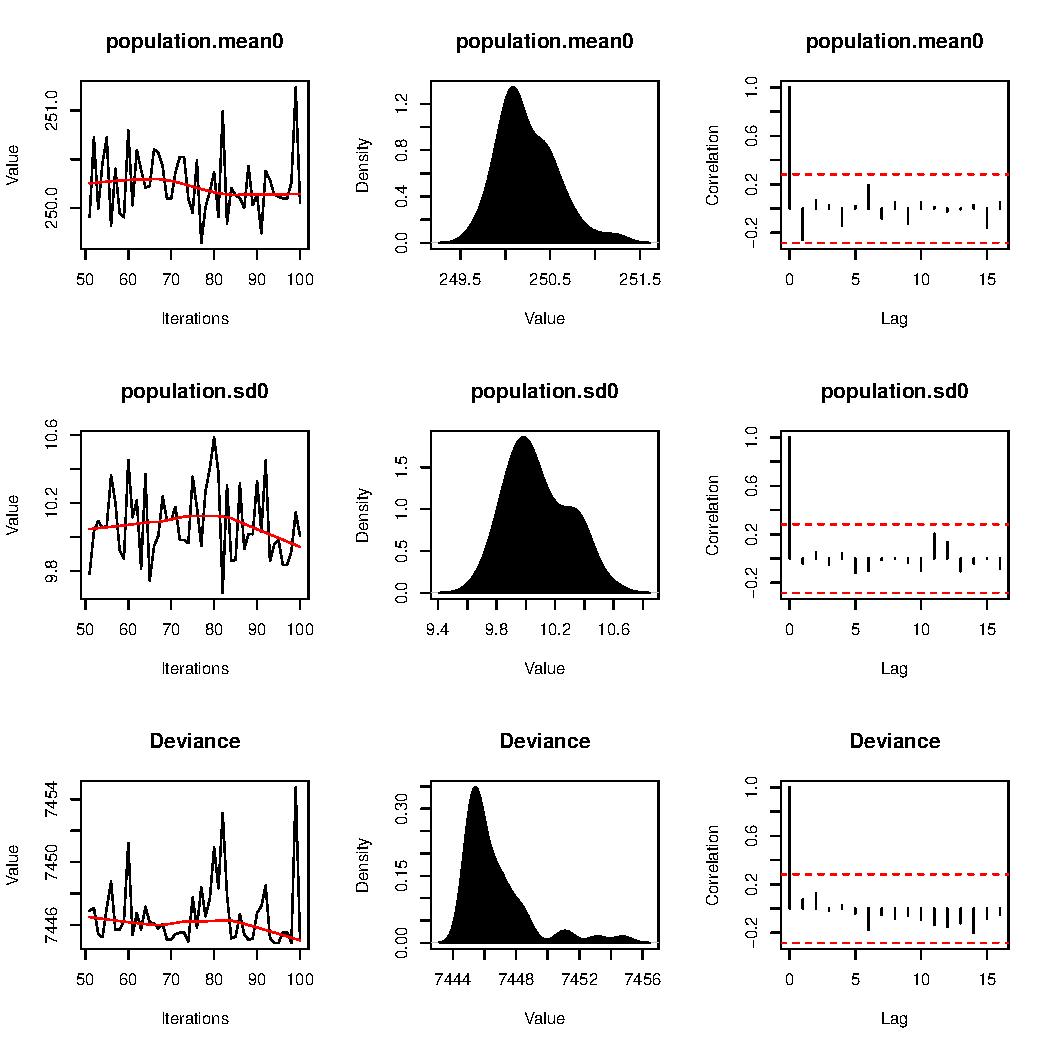
\includegraphics[width=\maxwidth]{figure/unnamed-chunk-132} 

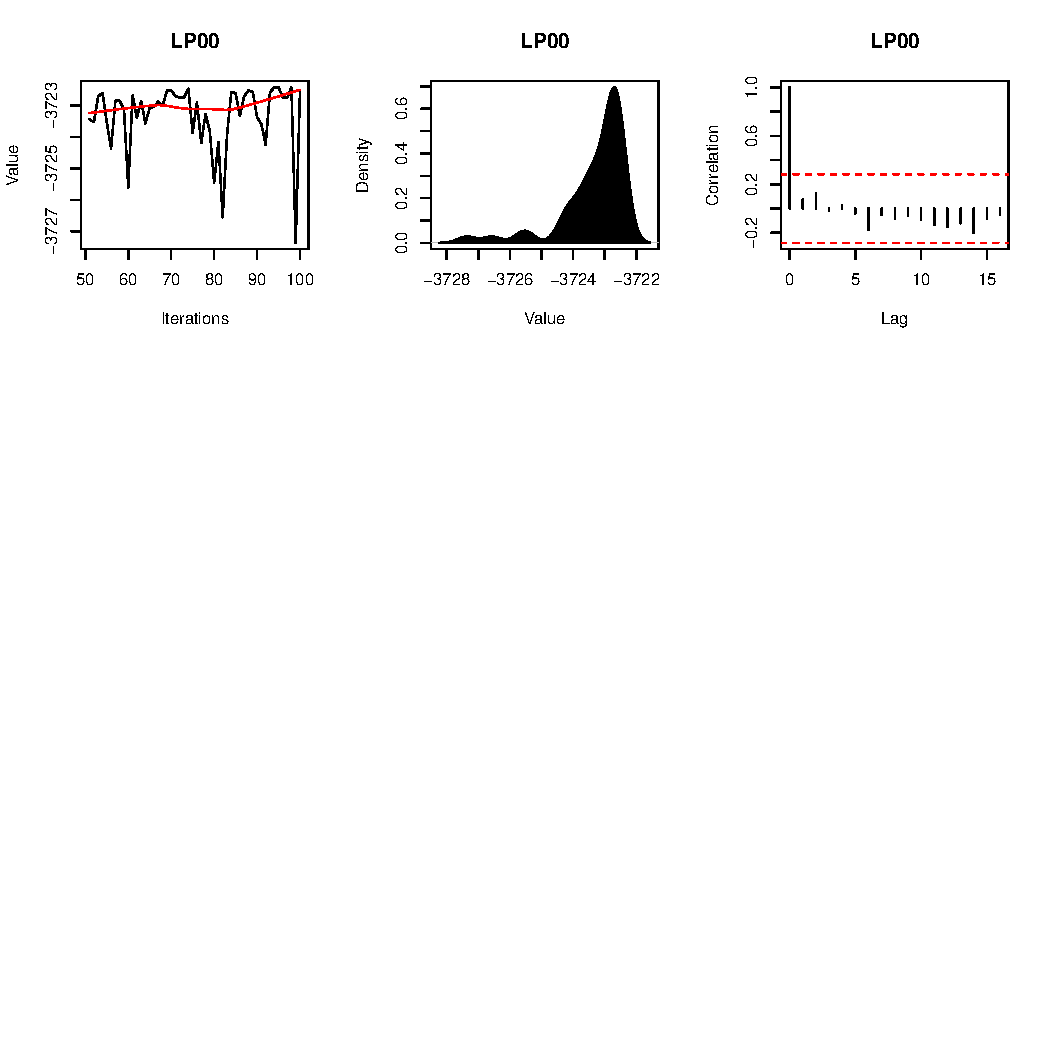
\includegraphics[width=\maxwidth]{figure/unnamed-chunk-133} 

\end{knitrout}


\end{document}














